%% CLI-First (arXiv v2.3, 2026-10-11; v2.3 fixes the errors the v2.2 review panel found): adds Section 7, three follow-up waves (revised after the v2 review panel;
%% readability pass: shorter captions, Figures 1-5 redrawn or added, full tables in the appendix)
%% ACM sigconf; nonacm for the preprint.
\documentclass[sigconf,nonacm]{acmart}

\usepackage{tikz}
\usetikzlibrary{positioning,arrows.meta,calc,fit,backgrounds}
\usepackage{pgfplots}
\usepackage{catchfile}
\pgfplotsset{compat=1.18}
\usepackage{booktabs}
\usepackage{tabularx}
%% acmart sets whole captions in bold for sigconf; keep the label and the lead bold only.
\captionsetup{textfont=normalfont}

%% The product's name is a macro so it can be anonymised in one place.
\newcommand{\sysA}{Salli}
\newcommand{\flag}[1]{\texttt{-\/-#1}}
\newcommand{\cmd}[1]{\texttt{#1}}
\newcommand{\cfg}[1]{\textsf{#1}}
\newcommand{\finding}[1]{\textbf{#1}}

%% One colour per protocol, used in every figure.
\definecolor{mcpc}{RGB}{37,99,165}
\definecolor{clic}{RGB}{212,106,20}

\settopmatter{printacmref=false}
\renewcommand\footnotetextcopyrightpermission[1]{}
\pagestyle{plain}
\setlength{\emergencystretch}{3em}

\newsavebox{\loopbox}
\newsavebox{\mcpbox}

\begin{document}

\title{CLI-First: What an Agent Knows About an Interface Matters More Than Its Protocol}

\author{Chandra Irugalbandara}
\affiliation{%
  \institution{Leaf Monkey Labs}
  \city{Colombo}
  \country{Sri Lanka}}
\email{chandra@leafmonkey.org}

\begin{abstract}
Coding agents now build and operate much of the software they touch, mostly from a terminal. We propose CLI-first development: a capability is done only when it works from the product's command-line interface (CLI), and that CLI is the reference client against which the other clients are checked. In a personal-finance product that adopted the rule, coverage fell behind until a dedicated phase restored it, and an agent's pass through the CLI found a safety control that held only on the web path. We then test a popular claim: that CLIs cost agents less than Model Context Protocol (MCP) servers. In 704 runs on one product, we varied the protocol, what the agent knew about the interface, and whether it could compose operations. Knowledge mattered more than protocol. Agents that learned the CLI from its help cost 1.6 to 2 times as much as agents given the curated MCP server. With a compact command sheet, the CLI could not be told apart from the server on chains of dependent steps for the stronger model. Composed, it cost 36 to 39\% less on two tasks that repeat an operation, at the price of coarser oversight. In 1{,}440 follow-up runs, the parts of the sheet that mattered depended on the model. On the product's rewritten version, the composed CLI with a sheet cost less than its MCP server, partly because that server had grown.
\end{abstract}

\begin{CCSXML}
<ccs2012>
<concept><concept_id>10003120.10003121.10003124</concept_id><concept_desc>Human-centered computing~Interaction paradigms</concept_desc><concept_significance>500</concept_significance></concept>
<concept><concept_id>10011007.10011074.10011099</concept_id><concept_desc>Software and its engineering~Software verification and validation</concept_desc><concept_significance>300</concept_significance></concept>
<concept><concept_id>10010147.10010178.10010219.10010221</concept_id><concept_desc>Computing methodologies~Intelligent agents</concept_desc><concept_significance>300</concept_significance></concept>
</ccs2012>
\end{CCSXML}
\ccsdesc[500]{Human-centered computing~Interaction paradigms}
\ccsdesc[300]{Software and its engineering~Software verification and validation}
\ccsdesc[300]{Computing methodologies~Intelligent agents}

\keywords{AI agents, command-line interfaces, Model Context Protocol, tool use, agent-computer interfaces, cost, oversight}

%% --- Teaser: one task solved both ways -----------------------------------
\begin{lrbox}{\mcpbox}\begin{minipage}[t]{0.40\textwidth}\scriptsize\ttfamily
get\_trial\_balance()\\
get\_accounts()\\
create\_reminder("Review spending: General Expenses", "2026-04-30")\\
create\_reminder("Review spending: Fuel", "2026-04-30")\\
create\_reminder("Review spending: Pharmacy", "2026-04-30")\\
\textrm{\itshape\dots{} and 21 more \texttt{create\_reminder} calls}\par\vspace{3mm}\noindent

\begin{tikzpicture}[x=2.6mm, y=1mm]
\foreach \i in {0,1} \fill[black!40] (\i,0) rectangle +(0.72,3.4);
\foreach \i in {2,...,25} \fill[mcpc] (\i,0) rectangle +(0.72,3.4);
\end{tikzpicture}\par\vspace{1mm}
{\rmfamily\footnotesize 26 tool calls, one operation each: 2 reads, then 24 writes}
\end{minipage}\end{lrbox}
\begin{lrbox}{\loopbox}\begin{minipage}[t]{0.47\textwidth}\scriptsize
\begin{verbatim}
# call 1
salli accounts list --json > $TMPDIR/a.json 2>/dev/null
salli ledger trial-balance --json > $TMPDIR/tb.json
jq -r --slurpfile tb $TMPDIR/tb.json '.[]
  | select(.type=="expense") | [.id,.name,.currency,
    ($tb[0][.id]//"none")] | @tsv' $TMPDIR/a.json
# call 2
jq -r --slurpfile tb $TMPDIR/tb.json '.[]
  | select(.type=="expense" and .currency=="LKR")
  | select((($tb[0][.id]//"0")|tonumber)>20000)
  | .name' $TMPDIR/a.json |
while IFS= read -r n; do salli reminders add \
  "Review spending: $n" --due-date 2026-04-30 --json; done
\end{verbatim}\vspace{-1.2mm}\noindent

\begin{tikzpicture}[x=2.6mm, y=1mm]
\fill[black!40] (0,0) rectangle +(0.72,3.4);
\fill[clic] (1,0) rectangle +(0.72,3.4);
\end{tikzpicture}\par\vspace{1mm}
{\footnotesize 2 tool calls: one reads and filters, one loops over the 24 writes}
\end{minipage}\end{lrbox}

\begin{teaserfigure}
\centering
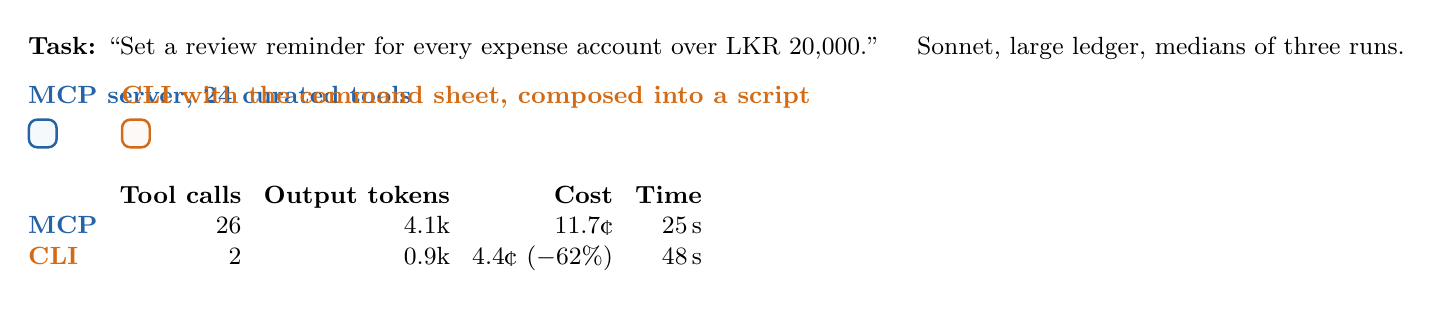
\begin{tikzpicture}[
  panel/.style={draw=#1, line width=0.9pt, rounded corners=3pt, inner sep=5pt, fill=#1!4},
  head/.style={font=\small\bfseries, text=#1, anchor=south west, inner xsep=0pt}]
\node[panel=mcpc] (m) {\usebox{\mcpbox}};
\node[head=mcpc] (mh) at (m.north west) {MCP server, 24 curated tools};
\node[panel=clic, right=8mm of m.north east, anchor=north west] (c) {\usebox{\loopbox}};
\node[head=clic] at (c.north west) {CLI with the command sheet, composed into a script};
\node[anchor=south west, font=\small, inner xsep=0pt] at ([yshift=1mm] mh.north west) {\textbf{Task:} ``Set a review reminder for every expense account over LKR 20{,}000.'' \quad Sonnet, large ledger, medians of three runs.};
\node[anchor=north west, font=\small, inner xsep=0pt] at ([yshift=-3mm] m.south west) {%
\setlength{\tabcolsep}{4pt}\begin{tabular}{@{}lrrrr@{}}
 & \textbf{Tool calls} & \textbf{Output tokens} & \textbf{Cost} & \textbf{Time} \\
\textcolor{mcpc}{\textbf{MCP}} & 26 & 4.1k & 11.7\textcent & 25\,s \\
\textcolor{clic}{\textbf{CLI}} & 2 & 0.9k & 4.4\textcent{} ($-$62\%) & 48\,s \\
\end{tabular}};
\end{tikzpicture}
\caption{\textbf{One CLI script replaced 26 MCP tool calls.} This is the cell where composition saved most; over both repetition tasks the saving was 36--39\%, and on chains, CLI agents without the command sheet cost more than MCP (Section~\ref{sec:f1}). Left: an abridged trace. Right: one run's two calls, with line breaks added.}
\label{fig:teaser}
\Description{A task banner reads: set a review reminder for every expense account over LKR 20,000; Sonnet, large ledger, medians of three runs. Two panels follow. Left, outlined in blue, MCP server with 24 curated tools: a list of tool calls, get_trial_balance, get_accounts, then create_reminder calls for General Expenses, Fuel and Pharmacy and 21 more, above a strip of 26 small bars, 2 grey reads and 24 blue writes. Right, outlined in orange, the CLI with the command sheet composed into a script: two shell commands; the first saves the account list and trial balance to files and lists expense accounts with jq, the second filters expense accounts over 20,000 with jq and loops over the names calling salli reminders add; below, a strip of 2 bars. A table underneath compares them: tool calls 26 against 2, output tokens 4.1k against 0.9k, cost 11.7 cents against 4.4 cents (62 percent less), time 25 seconds against 48 seconds.}
\end{teaserfigure}

\maketitle

%% ===========================================================================
\section{Introduction}

Agents are becoming a large share of the users of developer tools. Cloudflare reports that agents accounted for a quarter of the use of its command-line tool in March 2026, up from single digits a year earlier, and for 48\% by late September~\cite{cloudflare2026cf}. Inside product teams the shift shows in version control: in \sysA{}, the personal-finance product we study, 75\% of commits carry a coding agent's co-authorship trailer. Those agents need to run the software they change, not just compile it.

We propose \emph{CLI-first development}, a process with two rules: a capability is done only when it works from the product's command-line interface (CLI), and the CLI is the \emph{reference client} that the product's other clients, including the web application and any Model Context Protocol (MCP) server, are checked against. The proposal makes two claims. One concerns process: a CLI held to these rules lets the agents that build a product exercise and verify all of it. We examine it in \sysA{}'s version history. The other concerns cost and is widely argued, while the few measurements disagree: that a CLI is cheaper for agents than an MCP server because MCP loads every tool definition into the model's context~\cite{schmitt2026circleci,qi2026ibm}, or more expensive because every call starts a process~\cite{mindstudio2026mcpcli}.

To test the cost claim we held one product fixed and varied only the interface its agents used (Figure~\ref{fig:teaser}), crossing three factors: the \emph{protocol} (MCP tool calls or shell commands), what the agent \emph{knows} about the interface before it starts, and whether it may \emph{compose} operations into one program. If the interface did not matter, every configuration would cost what \sysA{}'s curated MCP server costs, and every ratio we report would be 1. What the agent knew moved cost more than the protocol did: on chains, replacing a CLI agent's help with a \emph{command sheet} (1.1k tokens of usage, options and output shapes, generated from the CLI) cut its cost relative to the server by more than the gap that remained between them. Our thesis follows: the case for CLI-first rests on the agents that build and check a product, and for agents in general, what they are told about an interface matters more than which protocol carries it. We report five findings from the main experiment and two from follow-ups:

\begin{itemize}
\item \finding{F1.} An agent that learned the CLI from its help cost 1.6 to 2 times as much as one given the curated MCP server's schemas (RQ1; Section~\ref{sec:f1}).
\item \finding{F2.} An MCP server generated from the CLI cost 1.3 to 1.8 times as much as the curated one, through both its larger catalogue and its larger results (RQ2; Section~\ref{sec:f2}).
\item \finding{F3.} With the command sheet and composition, the CLI could not be told apart from the curated server on chains for the stronger model, Sonnet, and cost 1.2 times as much for the weaker, Haiku (RQ3; Section~\ref{sec:f3}).
\item \finding{F4.} On two tasks that repeat an operation, the same configuration cost 36--39\% less than the curated server, including a one-write control cell where there was nothing to compose (RQ3; Section~\ref{sec:f4}).
\item \finding{F5.} Composition moved the unit a person could review from single actions to whole scripts, and agents on both protocols sometimes reported success they had not achieved (RQ4; Section~\ref{sec:f5}).
\item \finding{F6.} Which parts of the sheet mattered depended on the model: removing its options raised the weaker model's cost on chains and not the stronger model's (Section~\ref{sec:f6}).
\item \finding{F7.} On the product as rewritten since, the composed CLI with a sheet cost 0.60--0.90 times its MCP server on chains and 0.32--0.48 times on repetition tasks, partly because that server had doubled its catalogue; requiring account ids instead of codes made no detectable difference overall (Sections~\ref{sec:f7} and~\ref{sec:isolation}).
\end{itemize}

\noindent The paper contributes:
\begin{enumerate}
\item a definition of CLI-first development (Section~\ref{sec:principle});
\item a single-product case study of the rule in practice (Section~\ref{sec:cases});
\item a caching-aware cost model that separates what an interface costs an agent into description, discovery and composition (Section~\ref{sec:mcp});
\item an exploratory experiment and three follow-up waves, 2{,}144 runs in all, with every run, transcript and analysis released (Sections~\ref{sec:experiment} and~\ref{sec:followup});
\item principles for agent-ready CLIs, and controls for agents that act through them (Sections~\ref{sec:principles} and~\ref{sec:guardrails}).
\end{enumerate}

%% ===========================================================================
\section{Related Work}
\label{sec:related}

\paragraph{Delegation and oversight}
The debate between direct manipulation and delegation to agents is older than large language models~\cite{shneiderman1997direct,maes1994agents}. Norman warned that delegation works only when people keep an accurate sense of what the agent is doing and can take control back~\cite{norman1994agents}, and Horvitz's mixed-initiative principles~\cite{horvitz1999principles} and Amershi et al.'s guidelines for human-AI interaction~\cite{amershi2019guidelines} turn that concern into design advice. Work on automation describes how oversight degrades: the operator of a highly automated system is left with the hardest decisions and the least practice at them~\cite{bainbridge1983ironies}, the right level of automation differs by stage of a task~\cite{parasuraman2000model}, and trust has to be calibrated to reliability~\cite{lee2004trust}. An agent narrows the person's gulf of execution and can widen their gulf of evaluation~\cite{hutchins1985direct}, and stating intent is itself hard for non-experts~\cite{nielsen2023paradigm,zamfirescu2023johnny}. F5 bears on both gulfs.

\paragraph{Agent-computer interfaces and tool use}
SWE-agent showed that interface design changes agent performance: a purpose-built interface resolved 18.0\% of SWE-bench Lite tasks~\cite{jimenez2024swebench} against 11.0\% for a plain shell~\cite{yang2024sweagent}. CodeAct found that acting through executable code outperformed JSON and text tool calls by up to 20\% in success rate across 17 models~\cite{wang2024codeact}, and InterCode and Terminal-Bench evaluate agents in shells~\cite{yang2023intercode,merrill2026terminalbench}. Documentation alone lets models use unfamiliar tools about as well as demonstrations do~\cite{hsieh2023tooldoc}, and ReWOO and LLMCompiler cut model invocations by planning tool calls ahead~\cite{xu2023rewoo,kim2023llmcompiler}. Translating language into shell commands is a long-studied problem~\cite{lin2018nl2bash}.

\paragraph{GUI, API, CLI and MCP agents}
GUI agents beat CLI agents on 440 desktop tasks until the CLI's missing capabilities were filled in~\cite{zhou2026guicli}, and take 2.7 to 4.3 times more steps than necessary~\cite{abhyankar2025osworldhuman}; API-first and hybrid agents are faster~\cite{lu2024axis,zhang2025apigui,zhang2025ufo2}, and MCP tools raise computer-use agents' success~\cite{jia2025osworldmcp}. Comparisons of MCP and CLIs disagree. Across seven scaffoldings, paired MCP-to-CLI cost ratios ranged from 0.43 to 29~\cite{alier2026scaffolding}; in 120 runs MCP was 23\% faster and 2.5\% cheaper than an equivalent CLI~\cite{zechner2025mcpcli}. Two studies held a backend fixed. Smithery's 756 runs against public APIs found native MCP ahead of a CLI with descriptions on GitHub's REST API in success, tokens and time~\cite{mao2026smithery,nordicapis2026mcpcli}, and Scale Labs' 50 long-horizon tasks found that the CLI's advantage depended on model and task and mattered little for frontier models~\cite{hou2026scale}.

\paragraph{Practice and lineage}
``Agent experience'' has become a design concern~\cite{biilmann2025ax,baer2026agentsfirst}, and products increasingly give the UI and the agent one set of actions~\cite{builderio2026app,posthog2026golden}. For CLI input, named flags beat single JSON payloads on accuracy and cost~\cite{mastykarz2026dont,poehnelt2026rewrite}, and Mistral gives every interactive prompt a flag~\cite{mistral2026spaces}. The architecture underneath CLI-first is old: composable programs~\cite{mcilroy1978unix}, ports and adapters~\cite{cockburn2005hexagonal}, command-line design guidance~\cite{clig2020} and API usability research~\cite{myers2016api}; the decay of a shared interface is a form of architecture erosion~\cite{perry1992foundations,desilva2012erosion}. CLI-first differs from API-first in naming which client must work first and giving it the role of reference.

\paragraph{How this study differs}
Smithery's and Scale Labs' fixed-backend studies are closest to ours. We differ in three ways: (1) we vary what the agent knows about the interface and whether it may compose as separate factors, so their effects can be told apart; (2) we decompose cost by token type under prompt caching and model it, rather than reporting totals; and (3) we score a production product's database state rather than an agent's answer.

%% ===========================================================================
\section{CLI-First Development}
\label{sec:principle}

A team practises CLI-first development when it holds two rules:
\begin{description}
\item[R1, completeness.] A capability is done only when it works from the product's CLI. Other clients may ship it at the same time or later, but not instead.
\item[R2, reference.] The CLI is the reference client. When the web application, the MCP server or an embedded assistant disagrees with the CLI about what the product does, the disagreement is a defect in one of them, and checks written against the CLI define the expected behaviour.
\end{description}
R1 without R2 produces coverage that can drift; R2 without R1 produces a reference for part of the product.

Three kinds of agent use such a product (Figure~\ref{fig:arch}). Coding and operators' agents run in a shell and are the CLI's main users. Embedded agents call the same core operations and get no more power than any other client. Users' agents usually run where no shell exists and reach \sysA{} through an MCP server that OAuth binds to one user's data. CLI-first serves them only indirectly, by making every capability a scriptable operation that any protocol can expose; it does not guarantee that a protocol will: \sysA{}'s open-source core has 125 CLI commands but 24 MCP tools.

The analogy with mobile-first~\cite{wroblewski2009mobile,wroblewski2011mobile} holds for the order of work and fails on constraint: mobile-first started from the most limited client, CLI-first from the most capable, and its new user is an agent acting for a person. Accessibility is a closer precedent: the interfaces that expose an application to a screen reader stay complete only where teams treat gaps as defects.

\begin{figure}[t]
\centering
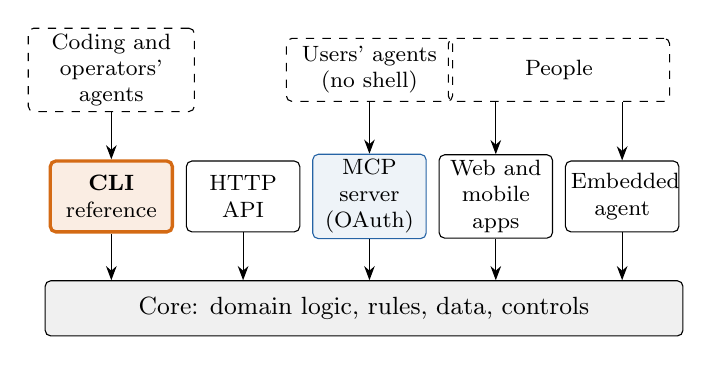
\begin{tikzpicture}[
  box/.style={draw, rounded corners=2pt, align=center, font=\footnotesize, minimum height=9mm, inner sep=2pt},
  surf/.style={box, minimum width=1.4cm, text width=1.3cm},
  cli/.style={box, draw=clic, fill=clic!12, very thick, minimum width=1.55cm, text width=1.4cm},
  mcps/.style={surf, draw=mcpc, fill=mcpc!8},
  core/.style={box, fill=black!6, minimum width=8.1cm, minimum height=7mm, font=\small},
  agent/.style={box, dashed, minimum height=8mm, inner xsep=3pt},
  >={Stealth[length=1.8mm]}
]
\node[cli] (cli) {\textbf{CLI}\\reference};
\node[surf, right=1.5mm of cli] (api) {HTTP API};
\node[mcps, right=1.5mm of api] (mcp) {MCP server\\(OAuth)};
\node[surf, right=1.5mm of mcp] (gui) {Web and\\mobile apps};
\node[surf, right=1.5mm of gui] (emb) {Embedded\\agent};
\node[core, below=6mm of $(cli.south west)!0.5!(emb.south east)$] (core) {Core: domain logic, rules, data, controls};
\foreach \s in {cli,api,mcp,gui,emb} { \draw[->] (\s.south) -- (\s.south |- core.north); }
\node[agent, text width=1.9cm, above=6mm of cli] (coding) {Coding and operators' agents};
\node[agent, text width=1.9cm] (users) at (mcp |- coding) {Users' agents (no shell)};
\coordinate (pc) at ($(gui)!0.5!(emb)$);
\node[agent, text width=2.6cm, minimum height=8mm] (people) at (pc |- coding) {People};
\draw[->] (coding) -- (cli);
\draw[->] (users) -- (mcp);
\draw[->] (people.south -| gui) -- (gui);
\draw[->] (people.south -| emb) -- (emb);
\end{tikzpicture}
\caption{\textbf{Every client calls one core; the CLI is the reference.} Dashed boxes: who uses each client.}
\label{fig:arch}
\Description{A diagram with a core at the bottom and five clients above it, each pointing down to the core: the CLI, highlighted in orange as the reference; the HTTP API; an MCP server with per-user OAuth access, in blue; the web and mobile apps; and an embedded agent. Above, in one row, coding and operators' agents point to the CLI, users' agents without a shell point to the MCP server, and people point to the apps and the embedded agent.}
\end{figure}

%% ===========================================================================
\section{A CLI-First Product}
\label{sec:cases}

\paragraph{Method}
We studied \sysA{}, a personal finance and tax product for Sri Lanka whose agent guidance adopts the CLI-first rule and which the author develops. The design is a single-case study with the author as participant-observer, in the tradition of autobiographical design~\cite{neustaedter2012autobiographical} and following case-study guidance from software engineering~\cite{runeson2009case}. The data are the product's git history (417 commits), architecture documents and commit messages at a fixed snapshot (13 September 2026). For CLI coverage we counted CLI commands and API route handlers, excluding authentication, at a series of dates; the ratio of counts is a proxy for parity, not a mapping of commands to routes. For agent involvement we counted commits whose message contains a \texttt{Co-Authored-By: Claude} trailer. The case can show what happened in one product; it cannot show how often CLI-first works elsewhere. Commit messages were themselves written with agent assistance and may be more explicit, and more favourable, than an independent record~\cite{bird2009git}.

\subsection{Coverage fell behind under a written rule and recovered in a dedicated phase}
\sysA{} combines a double-entry ledger, a versioned tax engine and AI agents that explain a user's financial position. Its domain core has no input/output or framework imports, and its CLI and HTTP API build their services through one composition function. The project's agent guidance states the order of work: ``Core + CLI first --- all domain logic runs from the terminal before any HTTP server exists,'' then the API, then web and mobile clients. 311 of its 417 commits carry an agent trailer.

\finding{The rule did not hold on its own.} An HTTP API with 19 feature routes existed from the first day, and over four weeks the API grew while the CLI did not: by 14 July the CLI had 13 commands against 54 feature routes, a ratio of 0.24 (Figure~\ref{fig:parity}). The roadmap then inserted a ``CLI completion'' phase ahead of new domain work, and within two days the ratio reached 0.82. Five domains built immediately afterwards each received core logic, API routes and a CLI command group within about twelve minutes, in one agent session. Coverage then fell to 0.73 as the API gained routes the CLI did not; the open-source core now runs a continuous-integration check that fails when a route has neither a command nor a recorded reason for lacking one. We have no data yet on whether the check holds coverage.

\begin{figure}[t]
\centering
\begin{tikzpicture}
\begin{axis}[width=\columnwidth, height=4.6cm, xmin=0, xmax=90, ymin=0, ymax=140, clip=false,
  xtick={0,28,56,84}, xticklabels={18 Jun, 16 Jul, 13 Aug, 10 Sep}, ytick={0,50,100}, ylabel={Count},
  tick label style={font=\footnotesize}, label style={font=\footnotesize}, axis lines*=left]
\fill[clic!12] (axis cs:26,0) rectangle (axis cs:28,140);
\draw[black!45, densely dashed] (axis cs:31,0) -- (axis cs:31,140);
\node[font=\footnotesize, text=clic, anchor=south west, align=left, inner sep=1pt] at (axis cs:2,104) {CLI completion\\phase \rlap{$\rightarrow$}};
\node[font=\footnotesize, text=black!65, anchor=north west, align=left, inner sep=1pt] at (axis cs:32.5,72) {19 Jul: CLI pass finds\\the approval gate open};
\addplot[thick, mark=none, color=black!70] table[x=day, y=api_feature_routes, col sep=comma] {data/salli_coverage.csv};
\addplot[thick, mark=*, mark size=1pt, color=clic] table[x=day, y=cli_commands, col sep=comma] {data/salli_coverage.csv};
\node[font=\footnotesize, text=black!70, anchor=south east] at (axis cs:87,129) {API feature routes};
\node[font=\footnotesize, text=clic, anchor=south east] at (axis cs:87,96) {CLI commands};
\node[font=\footnotesize, anchor=south] at (axis cs:13,15) {0.24};
\node[font=\footnotesize, anchor=north west] at (axis cs:28.5,88) {0.82};
\node[font=\footnotesize, anchor=north east] at (axis cs:87,88) {0.73 by Sep};
\end{axis}
\end{tikzpicture}
\caption{\textbf{CLI coverage fell under a written rule until a dedicated phase restored it.} Numbers: CLI commands per API feature route. Authentication routes excluded.}
\label{fig:parity}
\Description{A line chart over \sysA{}'s first 87 days, from 18 June to 13 September 2026. API feature routes, in grey, rise from 19 to 128; CLI commands, in orange, stay at 13 until day 27, jump to 89 by day 28 and reach 93. A shaded band marks the CLI completion phase on days 26 to 28, and a dashed line on 19 July marks the CLI pass that found the approval gate open. Labels give commands per route: 0.24 before the phase, 0.82 after it, and 0.73 by September.}
\end{figure}

\subsection{A pass through the CLI found a control that held on only one path}
Once the CLI covered the product, a coding agent's pass through it found defects in the core; one agent-assisted commit (\texttt{862ed06}, 19 July) records the defects ``found during a full CLI end-to-end pass''. The most serious was a control that held on only one path. The CLI had never set up the checkpointer that the HTTP server configures for the embedded agents, so the human-approval gate on their write tools silently did nothing when invoked from the CLI. The web client could not show this, because it reached the agents through the HTTP server, and the gate had been fixed for that path a month earlier. The same pass found that the agents' history commands crashed, that data export crashed for any user who had computed their tax, and that a command posting imported transactions misreported how many it had posted. These observations, from one product and one participant-observer, motivate study S2 in Section~\ref{sec:agenda}.

%% ===========================================================================
\section{What an Interface Costs an Agent}
\label{sec:mcp}

An MCP server publishes typed tools whose definitions the agent's host loads into the model's context~\cite{mcp2024spec}; the model calls tools one response at a time, possibly several in parallel. With a CLI that emits structured output, an agent can instead write a chain of operations once as a program and run it as one tool call, so that intermediate data move through pipes or files rather than through the model, as in Figure~\ref{fig:teaser}.

\paragraph{A cost model}
Consider $k$ operations, each needing the result of the one before. Let $S$ be the fixed prompt prefix (system prompt and interface description), $u$ the user's request, $a_i$ and $r_i$ the tokens of the $i$-th call and its result, $c$ the tokens of a pipeline script and $f$ its filtered output. With direct calls there are $k+1$ model passes, and pass $j$ reads $P_j = S + u + \sum_{i<j}(a_i + r_i)$. Without caching, the input tokens processed are
\begin{equation}
I_{\text{calls}} = (k+1)(S+u) + \sum_{i=1}^{k}(k+1-i)(a_i+r_i),
\label{eq:calls}
\end{equation}
quadratic in $k$ when results are of similar size, while a single pipeline needs two passes:
\begin{equation}
I_{\text{pipe}} = 2(S+u) + c + f.
\label{eq:pipe}
\end{equation}
With prompt caching, cache writes cost $\omega$ times the base input rate and cache reads $\rho$ times; for one provider $\rho = 0.1$, $\omega$ is 1.25 for five-minute and 2 for one-hour entries, and output costs five times the input rate~\cite{anthropic2026caching}. In input-token equivalents, direct calls and the pipeline then cost approximately
\begin{align}
C_{\text{calls}} &= \omega P_1 + \rho \textstyle\sum_{j\le k} P_j + \omega \sum_{i} (a_i + r_i), \label{eq:ccalls}\\
C_{\text{pipe}} &= \omega (S+u+c+f) + \rho (S+u) \label{eq:cpipe}
\end{align}
(Table~\ref{tab:cost}). Caching removes most of the quadratic term but not the $k+1$ sequential passes, nor the cost of every intermediate result entering the context once. When many agents share a prefix, even the first pass may read $S$ from the cache.

\begin{table}[t]
\caption{\textbf{A pipeline needs two passes where direct calls need $k+1$; caching narrows the gap but does not close it.} Input-token equivalents for $k=5$ dependent operations.}
\label{tab:cost}
\small
\begin{tabular}{@{}lrrr@{}}
\toprule
 & \textbf{Passes} & \textbf{Uncached} & \textbf{Cached} \\
\midrule
Direct tool calls & 6 & 97.5k & 34.5k \\
CLI pipeline & 2 & 22.6k & 15.6k \\
CLI pipeline, $S=1$k & 2 & 4.6k & 3.5k \\
\bottomrule
\end{tabular}

\smallskip\footnotesize $S=10$k, $u=1$k, $a_i=100$, $r_i=2$k, $c=400$, $f=200$, $\rho=0.1$, $\omega=1.25$ (the five-minute rate; the experiment used one-hour entries, $\omega=2$). Last row: no tool definitions in the prefix.
\end{table}

\paragraph{Discovery}
Two further terms decide whether a pipeline is available. The first is \emph{discovery}. Equation~\ref{eq:pipe} assumes an agent that knows the commands and the shape of their output. An MCP server supplies that knowledge in $S$; an agent that must learn a CLI reads help instead, taking $d$ extra passes that add $h$ tokens, written to the cache once and re-read on every later pass. Whether this exceeds the CLI's saving in $S$ depends on $d$, $h$ and the passes that follow.

\paragraph{Repetition}
The second is \emph{repetition}. For $n$ independent operations of one kind, direct calls can run in parallel within one pass, but the model writes all $n$ calls and all $n$ results enter the context. A loop over a CLI command avoids the per-call overhead; its length is constant in $n$ when it iterates over the product's own data, as in Figure~\ref{fig:teaser}, and grows with $n$ when the arguments must be written out.

\paragraph{Research questions}
\label{sec:hypotheses}
The model raises four questions. We formed the predictions after the first collection wave of the experiment (Section~\ref{sec:history}) and test them on data that include that wave, so they are exploratory.
\begin{description}
\item[RQ1, knowledge.] Does an agent that must learn a CLI from its help cost more than one given an MCP server's schemas? \emph{Predicted: yes.}
\item[RQ2, description size.] For the same operations, does an MCP server generated from the CLI cost more than a curated one? \emph{Predicted: yes.}
\item[RQ3, composition.] When the agent knows the commands, does a composed CLI cost less than the curated MCP server on chains of dependent operations, and on tasks that repeat an operation? \emph{Predicted: yes, more so for repetition.}
\item[RQ4, oversight.] What does composition do to what a person can review? \emph{No prediction.}
\end{description}

\paragraph{What composition costs}
Composition's economics come from code as the agent's action space, not from the shell; MCP tools can also be called from code in a sandbox~\cite{anthropic2025codeexec,anthropic2025advancedtools,cloudflare2025codemode}, though standard MCP clients do not offer it. A CLI brings composition with the interface, and with it five costs: scripts must anticipate output shapes that MCP declares; chains can fail halfway; shell quoting is fragile~\cite{mastykarz2026dont}; every invocation starts a process; and a shell carries ambient authority. A pipeline planned before reading data keeps untrusted content out of the control flow~\cite{debenedetti2025camel}; one that interpolates data into commands, like Figure~\ref{fig:teaser}'s loop, does not.

%% ===========================================================================
\section{An Exploratory Experiment}
\label{sec:experiment}

\subsection{Design}
We held one product, its data and its tasks fixed and varied the interface. The product was \sysA{}'s open-source core at commit \texttt{0277747}, whose CLI (125 commands, 120 with \flag{json}) and MCP server (24 tools) call the same services and database. A \emph{configuration} fixes three factors (Table~\ref{tab:arms}):
\begin{description}
\item[Protocol:] MCP tool calls or shell commands.
\item[Knowledge:] what the interface description tells the agent before it starts. MCP configurations receive tool schemas: \cfg{MCP-24} is the core's own, curated server, whose results are compact summaries; \cfg{MCP-102} is generated from the CLI, with one tool for each of 102 of the 120 commands that support \flag{json} (administrative command groups are left out), and returns the CLI's JSON, so it differs from \cfg{MCP-24} in both catalogue size and result size. CLI configurations receive help alone; the core's agent skill, pasted into the prompt (646 tokens naming command groups and rules, but no options); the core's five skills, installed for the agent to load if it chooses; or a \emph{command sheet} generated from the CLI's own definitions (1{,}134 tokens giving usage, options and JSON output shape for the 14 commands that do what \cfg{MCP-24}'s tools do).
\item[Composition:] whether the agent may combine commands. One-per-call configurations (\cfg{/step}) permitted only the \cmd{salli} executable; composed ones (\cfg{/comp}) asked the agent to compose dependent steps and allowed pipes, \cmd{jq}, scripts and, from collection wave 4, Python.
\end{description}

\finding{What the experiment can and cannot show.} It compares these configurations on one product, six tasks and two models from one provider. It cannot say how often CLIs beat MCP servers in general, and it does not test the process claim of Section~\ref{sec:cases}.

\begin{table}[t]
\caption{\textbf{Eight configurations cross protocol, knowledge and composition.} Each cell: a configuration, the median context of its first model call, and its retained runs.}
\label{tab:arms}
\footnotesize
\setlength{\tabcolsep}{3pt}
\begin{tabular}{@{}>{\raggedright\arraybackslash}p{2.7cm}>{\raggedright\arraybackslash}p{2.5cm}>{\raggedright\arraybackslash}p{2.5cm}@{}}
\toprule
\textbf{Knowledge} & \textbf{One operation per call} & \textbf{Composed} \\
\midrule
MCP: 24 curated schemas, 3.0k & \textcolor{mcpc}{\cfg{MCP-24}}\newline 5.3k; 96 runs & -- \\
MCP: 102 generated schemas, 9.7k & \textcolor{mcpc}{\cfg{MCP-102}}\newline 17.2k; 96 & -- \\
\midrule
CLI: help only & -- & \textcolor{clic}{\cfg{CLI help/comp}}\newline 2.9k; 64, chains only \\
CLI: skill in the prompt, 0.6k & \textcolor{clic}{\cfg{CLI skill/step}}\newline 3.8k; 64, chains only & \textcolor{clic}{\cfg{CLI skill/comp}}\newline 3.9k; 96 \\
CLI: five skills, on demand & -- & \textcolor{clic}{\cfg{CLI installed/comp}}\newline 6.6k; 96 \\
CLI: command sheet, 1.1k & \textcolor{clic}{\cfg{CLI sheet/step}}\newline 4.7k; 96 & \textcolor{clic}{\cfg{CLI sheet/comp}}\newline 4.7k; 96 \\
\bottomrule
\end{tabular}

\smallskip\footnotesize Sizes in \texttt{o200k\_base} tokens; runs over both models. MCP calls may run in parallel within a pass.
\end{table}

\begin{figure*}[t]
\centering
\begin{tikzpicture}
\begin{axis}[xmode=log, scale only axis, width=6.3cm, height=5.1cm, xmin=0.2, xmax=4.4, ymin=-0.6, ymax=7.1, xtick={0.25,0.5,1,2,4}, xticklabels={0.25,0.5,1,2,4}, ytick={0,...,6}, tick label style={font=\footnotesize}, label style={font=\footnotesize}, title style={font=\small}, xlabel={Cost relative to \cfg{MCP-24} (log scale; lower is cheaper)}, title={(a) Chains, $k\in\{1,2,4,8\}$}, yticklabels={CLI sheet/comp, CLI sheet/step, CLI installed/comp, CLI skill/comp, CLI skill/step, CLI help/comp, MCP-102}, legend style={font=\footnotesize, at={(0.98,0.02)}, anchor=south east, draw=none, fill=white, fill opacity=0.9, text opacity=1}]
\fill[black!5] (axis cs:0.2,-0.6) rectangle (axis cs:1,7.1);
\draw[black!18] (axis cs:0.2,5.5) -- (axis cs:4.4,5.5); \draw[black!18] (axis cs:0.2,4.5) -- (axis cs:4.4,4.5); \draw[black!18] (axis cs:0.2,1.5) -- (axis cs:4.4,1.5);
\draw[black!55, dashed] (axis cs:1,-0.6) -- (axis cs:1,7.1);
\node[font=\footnotesize, text=black!60, anchor=west] at (axis cs:1.03,6.78) {\cfg{MCP-24} = 1};
\addplot[forget plot, draw=none, mark=none, mcpc!45, error bars/.cd, x dir=both, x explicit] table[x=ratio, y=y, x error plus=tplus, x error minus=tminus, col sep=comma] {data/pilot/forest_chain_haiku_mcp.csv};
\addplot[forget plot, draw=none, mark=none, clic!45, error bars/.cd, x dir=both, x explicit] table[x=ratio, y=y, x error plus=tplus, x error minus=tminus, col sep=comma] {data/pilot/forest_chain_haiku_cli.csv};
\addplot[forget plot, draw=none, mark=none, mcpc!45, error bars/.cd, x dir=both, x explicit] table[x=ratio, y=y, x error plus=tplus, x error minus=tminus, col sep=comma] {data/pilot/forest_chain_sonnet_mcp.csv};
\addplot[forget plot, draw=none, mark=none, clic!45, error bars/.cd, x dir=both, x explicit] table[x=ratio, y=y, x error plus=tplus, x error minus=tminus, col sep=comma] {data/pilot/forest_chain_sonnet_cli.csv};
\addplot[forget plot, only marks, mark=o, mark size=1.9pt, thick, mcpc, error bars/.cd, x dir=both, x explicit, error bar style={line width=1.3pt}] table[x=ratio, y=y, x error plus=plus, x error minus=minus, col sep=comma] {data/pilot/forest_chain_haiku_mcp.csv};
\addplot[forget plot, only marks, mark=o, mark size=1.9pt, thick, clic, error bars/.cd, x dir=both, x explicit, error bar style={line width=1.3pt}] table[x=ratio, y=y, x error plus=plus, x error minus=minus, col sep=comma] {data/pilot/forest_chain_haiku_cli.csv};
\addplot[forget plot, only marks, mark=square*, mark size=1.7pt, mcpc, error bars/.cd, x dir=both, x explicit, error bar style={line width=1.3pt}] table[x=ratio, y=y, x error plus=plus, x error minus=minus, col sep=comma] {data/pilot/forest_chain_sonnet_mcp.csv};
\addplot[forget plot, only marks, mark=square*, mark size=1.7pt, clic, error bars/.cd, x dir=both, x explicit, error bar style={line width=1.3pt}] table[x=ratio, y=y, x error plus=plus, x error minus=minus, col sep=comma] {data/pilot/forest_chain_sonnet_cli.csv};
\addlegendimage{only marks, mark=o, mark size=1.9pt, black, thick}\addlegendentry{Haiku}
\addlegendimage{only marks, mark=square*, mark size=1.7pt, black}\addlegendentry{Sonnet}
\end{axis}
\end{tikzpicture}\hfill
\begin{tikzpicture}
\begin{axis}[xmode=log, scale only axis, width=6.3cm, height=5.1cm, xmin=0.2, xmax=4.4, ymin=-0.6, ymax=7.1, xtick={0.25,0.5,1,2,4}, xticklabels={0.25,0.5,1,2,4}, ytick={0,...,6}, tick label style={font=\footnotesize}, label style={font=\footnotesize}, title style={font=\small}, xlabel={Cost relative to \cfg{MCP-24} (log scale; lower is cheaper)}, title={(b) Repetition: bulk entry and fan-out}, yticklabels={}]
\fill[black!5] (axis cs:0.2,-0.6) rectangle (axis cs:1,7.1);
\draw[black!18] (axis cs:0.2,5.5) -- (axis cs:4.4,5.5); \draw[black!18] (axis cs:0.2,4.5) -- (axis cs:4.4,4.5); \draw[black!18] (axis cs:0.2,1.5) -- (axis cs:4.4,1.5);
\draw[black!55, dashed] (axis cs:1,-0.6) -- (axis cs:1,7.1);
\node[font=\footnotesize, text=black!60, anchor=west] at (axis cs:1.03,6.78) {\cfg{MCP-24} = 1};
\node[font=\footnotesize, text=black!50, anchor=east] at (axis cs:0.95,5) {\itshape not run};
\node[font=\footnotesize, text=black!50, anchor=east] at (axis cs:0.95,4) {\itshape not run};
\addplot[forget plot, only marks, mark=o, mark size=1.9pt, thick, mcpc, error bars/.cd, x dir=both, x explicit, error bar style={line width=1.3pt}] table[x=ratio, y=y, x error plus=plus, x error minus=minus, col sep=comma] {data/pilot/forest_loop_haiku_mcp.csv};
\addplot[forget plot, only marks, mark=o, mark size=1.9pt, thick, clic, error bars/.cd, x dir=both, x explicit, error bar style={line width=1.3pt}] table[x=ratio, y=y, x error plus=plus, x error minus=minus, col sep=comma] {data/pilot/forest_loop_haiku_cli.csv};
\addplot[forget plot, only marks, mark=square*, mark size=1.7pt, mcpc, error bars/.cd, x dir=both, x explicit, error bar style={line width=1.3pt}] table[x=ratio, y=y, x error plus=plus, x error minus=minus, col sep=comma] {data/pilot/forest_loop_sonnet_mcp.csv};
\addplot[forget plot, only marks, mark=square*, mark size=1.7pt, clic, error bars/.cd, x dir=both, x explicit, error bar style={line width=1.3pt}] table[x=ratio, y=y, x error plus=plus, x error minus=minus, col sep=comma] {data/pilot/forest_loop_sonnet_cli.csv};
\end{axis}
\end{tikzpicture}
\caption{\textbf{Knowledge, more than protocol, decides cost; composition pays when work repeats.} Rows are grouped by what the agent knew; blue: MCP, orange: CLI. Thick bars: 95\% intervals for these tasks; thin bars: over tasks (chains only). The shaded side is cheaper than \cfg{MCP-24}.}
\label{fig:forest}
\Description{Two forest plots on a log scale with a dashed line at 1, the cost of MCP-24; the side below 1 is shaded as cheaper. Rows, top to bottom: MCP-102, CLI help/comp, CLI skill/step, CLI skill/comp, CLI installed/comp, CLI sheet/step and CLI sheet/comp. Left, chain tasks: MCP-102 sits near 1.6 to 1.8; the CLI configurations without the command sheet sit between 1.2 and 2.7; CLI sheet/step near 1.25; CLI sheet/comp at 1.21 for Haiku and 0.89 for Sonnet. Right, repetition tasks, where help/comp and skill/step were not run: MCP-102 near 1.3 to 1.5; CLI skill/comp around 0.64 to 0.79; CLI installed/comp around 1.1 to 1.2; CLI sheet/step at 1.15 for Haiku and 2.9 for Sonnet; CLI sheet/comp at 0.64 for Haiku and 0.61 for Sonnet.}
\end{figure*}

\paragraph{Tasks and scoring}
Six tasks could all be completed with the operations available to \cfg{MCP-24}:
\begin{itemize}
\item \emph{Chains} of $k = 1, 2, 4$ and $8$ dependent operations, with nominal depths 1, 2, 4 and 6: report the tax owed; record a cash expense; record a salary, compute the tax and set a reminder carrying the figure; and create an account, post to it, find the expense account with the largest balance, refund it, and set a reminder carrying the tax and the bank balance.
\item \emph{Repetition tasks}: record 25 expenses listed in the request (bulk entry), and set a reminder for every expense account over LKR~20{,}000 (fan-out, Figure~\ref{fig:teaser}).
\end{itemize}
Each ran on a small ledger (16 accounts, 30 entries) and a large one (106 accounts, 440 entries). Fan-out needs one write on the small ledger and 24 on the large, which makes the small cell a control where composition has nothing to compose. A \emph{cell} is one task on one ledger, so there are 12 cells and 24 combinations of model and cell. Every run used a freshly seeded user. The one-operation tax question was scored from the answer and the other tasks against the database, by the expected records; the $k=2$ and repetition tasks also required that no other records of the same kind exist on the task's dates, while the $k=4$ and $k=8$ checks did not look for extra records.

\paragraph{Interface asymmetries}
\cfg{MCP-24}'s reminder tool takes free text, while the CLI's \cmd{reminders add} takes it as a \texttt{KIND} argument that neither the skill nor the sheet explains. The CLI accepts account codes. The core's documentation, our prompt for the CLI configurations and the command sheet's header all said identifiers could be shortened to a unique prefix, which \cmd{entry add} did not accept. On the small ledger the $k=8$ task's target account is necessarily the one created in its first step.

\paragraph{Harness}
The agent was Claude Code 2.1.293 in headless mode driving Claude Haiku~5.5 and Claude Sonnet~5.5. Its system prompt was replaced by a short task prompt common to all configurations plus a configuration-specific paragraph; user settings were excluded, MCP tool search disabled, and only the configuration's tools enabled. The composed configurations' paragraph alone gave a reason to compose, so ``that intermediate output does not have to pass through you''; no other configuration was told anything about efficiency. The common prompt also said that the request was the user's confirmation for any change it asked for, so no configuration paused for approval. \cfg{MCP-24} ran the core's server over stdio with its OAuth user lookup replaced by the seeded user.

\paragraph{Permissions and caching}
Composed configurations ran with permissions bypassed under a deny-list of deletion, network, version-control and package-manager commands, and with a directory holding only \cmd{salli} prepended to the path; there was no sandbox, and the environment held the test instance's database URL and service keys. No transcript shows a command that bypassed the CLI. Caching used one-hour entries shared across runs: in 702 of 704 runs the first call read the prompt and interface description from a cache warmed by earlier runs.

\subsection{Collection history}
\label{sec:history}
\finding{The design grew in five collection waves, each started after the previous one's results were visible} (Appendix~\ref{app:history}). The first, a pilot on the chain tasks, found the CLI more expensive than \cfg{MCP-24}; the command-sheet configurations, the repetition tasks and the research questions came afterwards, and the pilot's 128 \cfg{MCP-24} and \cfg{CLI skill/step} runs are part of the analysed data. Of 947 runs attempted, 243 were superseded because of four harness problems and 704 retained; the run ledger lists each run's wave, parallelism, permissions and fate.

\subsection{Measures and analysis}
\label{sec:analysis}
For each run we recorded success; cost; tokens of each kind, summed over the run's agent invocations; passes, tool calls and characters of tool output; and time as reported by the agent harness, summed over invocations. Cost is at list prices: \$0.10, 0.20, 0.01 and 0.50 per million uncached input, cache-write, cache-read and output tokens for Haiku, and \$2, 4, 0.20 and 10 for Sonnet. These prices reproduce the harness's reported cost for every run.

\paragraph{Reading the results}
\begin{description}
\item[Ratio.] A configuration's cost relative to a baseline, \cfg{MCP-24} unless stated: in each cell the ratio of geometric-mean costs, combined over cells by the geometric mean. Below 1 is cheaper.
\item[For these tasks.] A 95\% Welch-type $t$ interval for the mean log ratio over cells, with runs within cells as the sampling unit and Satterthwaite degrees of freedom. A bootstrap over runs within cells~\cite{efron1994bootstrap} gives similar intervals and is in the released data.
\item[For tasks like these.] A 95\% $t$ interval over tasks, using each task's log ratio averaged over its two ledgers: wide with four chain tasks, uninformative with two repetition tasks.
\item[$p$.] A stratified permutation test (10{,}000 permutations), Holm-adjusted within each table~\cite{holm1979}; the smallest attainable value is 0.002. Bold in a table marks a Holm-adjusted $p < 0.05$.
\end{description}
We compare models as a ratio of ratios, overall and per task, and give absolute differences in cents.

\subsection{Results}
\label{sec:results}

\finding{Success was at ceiling, so cost decides.} Of 704 runs, 693 (98.4\%) succeeded; per configuration and model, success ranged from 95\% (57 of 60) to 100\%, with overlapping Wilson intervals. Figure~\ref{fig:forest} gives every cost ratio. Appendix~\ref{app:results} adds their $p$-values (Table~\ref{tab:effects}) and the median cost per run behind them (Table~\ref{tab:results}), from 0.05 to 70.9 cents.

\finding{On chains, the command sheet mattered more than composition.} Holding composition fixed, replacing help with the sheet lowered the chain ratio from 1.99 to 1.21 (Haiku) and from 1.62 to 0.89 (Sonnet); holding the sheet fixed, composition lowered it only from 1.28 to 1.21 and from 1.24 to 0.89. On repetition tasks composition did more, lowering the ratio from 1.15 to 0.64 and from 2.90 to 0.61. Knowledge thus moved cost most on chains (F1, F3), a generated MCP server cost more (F2), and composition paid on repetition tasks (F4) and coarsened oversight (F5).

\subsection{F1. Agents that learned the CLI from its help paid 1.6 to 2 times as much}
\label{sec:f1}
On chains, \cfg{CLI help/comp} cost about 0.2 and 1.7 cents more per task than \cfg{MCP-24} for Haiku and Sonnet, with intervals above 1 for these tasks and for tasks like these (RQ1); it cost more in all 8 cells for Haiku and 7 of 8 for Sonnet. These agents made two to four help calls per run, and at $k=8$ took a median of 15.5 passes against 7 for \cfg{MCP-24} (Haiku). A skill that named the command groups but no options did not close the gap (1.22 to 2.08). Installed skills were loaded in 35 of 60 Haiku and 30 of 36 Sonnet runs, arrived as an extra pass, and made \cfg{CLI installed/comp} the most expensive configuration on chains (2.74 and 1.95).

\subsection{F2. The generated MCP server cost more than the curated one in every cell}
\label{sec:f2}
\cfg{MCP-102} cost 1.79 and 1.57 times as much as \cfg{MCP-24} on chains with Haiku and Sonnet, and 1.53 and 1.34 times on repetition tasks, in all 12 cells for both models (RQ2; $p = 0.002$ throughout). Its schemas took 9.7k tokens against 3.0k, and it also returned 2.3 to 3.4 times as many characters of results. By the cost model, re-reading its larger catalogue accounts for a median of 16\% to 53\% of its extra cost, depending on model and task family, so its catalogue and its larger results both contributed. Against the CLI it was generated from, used with the command sheet and composed, it was the more expensive interface on both models and both task families.

\subsection{F3. With the sheet, chains cost about what MCP did for Sonnet and more for Haiku}
\label{sec:f3}
With the command sheet and composition, Sonnet's ratio, 0.89, was under a cent per task below \cfg{MCP-24}'s cost, but both its intervals include 1 (RQ3); Haiku's, 1.21, was about 0.07 cents above. Sonnet's ratio was 0.74 times Haiku's (0.67--0.82): at $k=8$ on the large ledger Sonnet composed the task into three tool calls and four passes, and Haiku into ten calls and nine passes.

\finding{The CLI's fuller results cost one-per-call agents more.} The CLI's JSON is fuller than \cfg{MCP-24}'s summaries. With one command per call, \cfg{CLI sheet/step} agents received about twice as many characters of results as \cfg{MCP-24}'s (1.98 times for Haiku, 1.96 for Sonnet) and cost 1.28 and 1.24 times as much, although, like \cfg{MCP-24}'s agents, they issued one operation per call. Composed agents could filter results before they reached the model, and received 1.64 and 1.07 times as many characters.

\subsection{F4. Composition paid when an operation repeated}
\label{sec:f4}
\finding{On the two repetition tasks, the composed CLI with the command sheet cost 36--39\% less than \cfg{MCP-24}} (RQ3): about 0.3 cents less per task with Haiku and 4 cents with Sonnet. Cost fell in three of four cells for Haiku and four of four for Sonnet.

\finding{The pooled saving includes a control cell.} By task, Haiku's ratios were 0.41 on bulk entry and 1.02 on fan-out, and Sonnet's 0.67 and 0.56, so the overall ratio of ratios, 0.95, hides an interaction between model and task. Haiku's fan-out ratio averages its 24-write cell, 0.61, with the one-write control, 1.70; leaving the control out, the composed CLI cost 0.46 times \cfg{MCP-24} for Haiku and 0.54 for Sonnet. In the control cell, the fan-out that needs one write, composition had nothing to compose and gave no consistent advantage: \cfg{MCP-24} was cheaper for Haiku (0.11 against 0.18 cents) and more expensive for Sonnet (1.83 against 1.61). Two tasks cannot establish generality; the interval over tasks spans 0.20 to 1.91 for Sonnet.

\finding{One command per call reversed the saving for Sonnet,} at 2.90 times \cfg{MCP-24}. On bulk entry its agents issued the 25 writes in parallel, with account identifiers shortened to a prefix as the documentation, our prompt and the command sheet said they could be; \cmd{entry add} rejected each with a traceback, the agents repeated the writes, and the two bulk cells cost 5.7 and 6.6 times \cfg{MCP-24}. Composition without the sheet had point estimates like the sheet's that were not established (\cfg{CLI skill/comp}, 0.79 for Haiku and 0.64 for Sonnet; Holm $p = 0.19$ and $0.067$), and restoring the superseded runs moves Sonnet's to 0.81.

\subsection{F5. Composition coarsened oversight, and neither protocol made reports reliable}
\label{sec:f5}
\finding{The configuration that saved most put 25 writes behind one tool call} (RQ4). With \cfg{MCP-24} or one command per call, each tool call carried at most one write; on the bulk task the composed agents placed a median of 25 writes in a single call. No person approved anything in the experiment, so this describes what a reviewer would be shown, not how reviewers would fare: per-action approval would become approval of a script. In 31 of the 96 composed repetition runs the script also sent the writes' output to \texttt{/dev/null}, so not even the transcript records what each write returned. \finding{Five of the 11 failures ended in a report of success}, 5 of 704 runs, as coded by the author. Two were with \cfg{MCP-24} (an omitted account; the wrong one of two similar names), one each with \cfg{MCP-102} and \cfg{CLI sheet/step} (each refunded the wrong account), and one with \cfg{CLI skill/comp} (reminder texts carrying stray quotation marks). One \cfg{MCP-24} agent ended: ``Created 23 reminders \dots{} for the expense accounts over LKR 20,000'', when 24 qualified. The other six failures disclosed what had gone wrong.

\subsection{Where the saving came from}
\label{sec:mechanism}
\finding{Composition saved tokens rather than passes.} Across the 24 combinations of model and cell, \cfg{CLI sheet/comp} took more passes than \cfg{MCP-24} in 8, fewer in 4 and as many in 12; its saving came from what each pass carried. Table~\ref{tab:mech} decomposes two Sonnet cells. On the $k=8$ chain, \cfg{CLI sheet/comp} read 36k cached tokens against 64k for \cfg{MCP-24}, and three quarters of its saving came from smaller cache writes; the help-only agent took twice the passes and read twice as much. \cfg{MCP-24} took 5 passes rather than $k+1 = 9$ because it issued independent calls in parallel. On the fan-out, smaller cache writes (54\%) and fewer output tokens (44\%) made up the saving; on Haiku's bulk task output tokens made up 63\%.

\begin{table}[t]
\caption{\textbf{The composed agent wrote less and re-read less.} Medians in two Sonnet cells on the large ledger.}
\label{tab:mech}
\CatchFileDef{\mechrows}{data/pilot/table_mech.tex}{}
\small
\setlength{\tabcolsep}{2.6pt}
\begin{tabular}{@{}lrrrrrr@{}}
\toprule
\textbf{Config.} & \textbf{Write, k} & \textbf{Read, k} & \textbf{Out, k} & \textbf{Passes} & \textbf{Calls} & \textbf{Cost, \textcent} \\
\midrule
\mechrows
\bottomrule
\end{tabular}
\end{table}

\subsection{Robustness, speed and failures}
\label{sec:robust}
\finding{The conclusions survive a cold cache and the superseded runs.} Re-pricing every run as if its first pass had written the cache raises \cfg{MCP-102}'s chain ratio to 2.44 and 2.38 and lowers \cfg{CLI help/comp}'s to 1.41 and 1.17. \cfg{CLI sheet/comp}'s ratios move by at most 0.11 and \cfg{CLI sheet/step}'s by up to 0.32; two ratios that were near 1 and not significant move just below it (\cfg{CLI skill/comp}, Sonnet, chains, 1.22 to 0.99; \cfg{CLI installed/comp}, Sonnet, repetition, 1.11 to 0.97). Restoring the superseded shared-directory runs changes no ratio by more than 0.08 except \cfg{CLI skill/comp} on Sonnet's repetition tasks, from 0.64 to 0.81.

\finding{The curated MCP server was fastest.} In time reported by the agent harness, \cfg{MCP-24} took a median of 9.5 seconds per run on chains (8.6 for Haiku, 11.5 for Sonnet), against 15.3 to 39.3 for the CLI configurations and 16.3 for \cfg{MCP-102}, which like the CLI starts a Python process per call. On repetition tasks it took 26.5 seconds, against 60.3 to 69.2 for every other configuration. Runs executed six to eight at a time in collection waves 1--4 and one at a time in wave 5.

\finding{The CLI failed in ways \cfg{MCP-24} did not.}
\begin{itemize}
\item Raw Python tracebacks of up to 9{,}400 characters entered the context in 48 of 512 CLI runs. In 30 they followed identifiers shortened to a prefix, which \cmd{entry add} rejected although the documentation and our command sheet said it would accept them; in 3 they followed account codes, in 11 values that the agents' scripts computed and the transcripts do not show, and in 4 we found no cause. Five \cfg{MCP-102} runs also met tracebacks, all after account codes, which that commit did not accept either.
\item Outputs over the harness's 30~KB limit were truncated to a preview in 56 CLI runs.
\item Five composed runs took 11.6 to 15.9 minutes: in two, a command the agent wrote waited on standard input until the harness moved it to the background; in two, the agent called the trial balance once per account; one we could not explain.
\end{itemize}
\cfg{MCP-24} met none of these problems.

%% ===========================================================================
\section{Three Follow-Up Waves}
\label{sec:followup}

After the first version of this paper we ran three follow-up waves (Table~\ref{tab:waves3}). The \emph{ablation wave} asks which parts of the command sheet mattered, the \emph{rewrite wave} runs the paper's tasks on the product as rewritten since, and the \emph{isolation wave} separates two of the rewrite's changes. All used the main experiment's harness, Claude Code version (2.1.293), models and statistics, and every run attempted was kept: 1{,}440 runs, of which 1{,}431 succeeded. Neither the questions nor the analyses were pre-registered, and in each wave the Sonnet runs followed the Haiku runs. Section~7's tests are Welch $t$-tests, Holm-adjusted within each table, not the permutation test of Section~\ref{sec:analysis}; intervals are unadjusted. The ablation and rewrite waves overlapped on one machine, so we do not compare their timings. Figure~\ref{fig:followup} shows the main results, and Appendix~\ref{app:followup} gives every ratio.

\begin{table*}[t]
\caption{\textbf{Three follow-up waves.} Each ran five Haiku and three Sonnet runs per cell, with the main experiment's harness, models, tasks and statistics.}
\label{tab:waves3}
\small
\begin{tabularx}{\textwidth}{@{}l l >{\raggedright\arraybackslash}X >{\raggedright\arraybackslash}X r >{\raggedright\arraybackslash}p{2.3cm}@{}}
\toprule
\textbf{Wave} & \textbf{Commit} & \textbf{Question} & \textbf{Configurations} & \textbf{Runs} & \textbf{Machine} \\
\midrule
Ablation (\S\ref{sec:f6}) & \texttt{0277747} & Which parts of the command sheet mattered? & \cfg{CLI sheet/comp} with five sheets; \cfg{MCP-24} & 576 (572) & shared with the rewrite wave \\
Rewrite (\S\ref{sec:f7}) & \texttt{1322f84} & Do the findings hold on the rewritten product? & \cfg{MCP-46}; \cfg{CLI help/comp}, \cfg{skill/comp}, \cfg{sheet/step}, \cfg{sheet/comp} & 480 (475) & shared with the ablation wave \\
Isolation (\S\ref{sec:isolation}) & \texttt{1322f84} & Did the server's growth or the CLI's account codes cause the change? & \cfg{MCP-46} with all 46 or only 24 tools; \cfg{CLI sheet/comp} with codes or with ids only & 384 (384) & alone, four runs at a time \\
\bottomrule
\end{tabularx}

\smallskip\footnotesize Runs: attempted (succeeded). Where two waves shared the machine, a median of 6 to 10 agents ran at once.
\end{table*}

\begin{figure*}[t]
\centering
\begin{tikzpicture}
\begin{axis}[xmode=log, scale only axis, width=4.15cm, height=3.3cm, ymin=-0.55, ymax=3.55, ytick={0,...,3}, yticklabels={Sonnet repetition, Sonnet chains, Haiku repetition, Haiku chains}, xmin=0.75, xmax=1.6, xtick={0.8,1,1.25,1.5}, xticklabels={0.8,1,1.25,1.5}, tick label style={font=\footnotesize}, label style={font=\footnotesize}, title style={font=\small, text width=4.15cm, align=center}, title={(a) Ablation: parts of the sheet removed}, xlabel={Cost with the element removed}, legend style={font=\footnotesize, draw=none, at={(0.5,-0.3)}, anchor=north, legend columns=1, row sep=-1pt}, legend cell align=left]
\draw[black!55, dashed] (axis cs:1,-0.55) -- (axis cs:1,3.55);
\draw[black!18] (axis cs:0.75,1.5) -- (axis cs:1.6,1.5);
\addplot[only marks, mark=*, mark size=1.8pt, clic, error bars/.cd, x dir=both, x explicit, error bar style={line width=1.1pt}] table[x=ratio, y=y, x error plus=plus, x error minus=minus, col sep=comma] {data/followup/fig_ablation_options.csv};
\addlegendentry{without options}
\addplot[only marks, mark=square, mark size=1.8pt, thick, clic, error bars/.cd, x dir=both, x explicit, error bar style={line width=1.1pt}] table[x=ratio, y=y, x error plus=plus, x error minus=minus, col sep=comma] {data/followup/fig_ablation_shapes.csv};
\addlegendentry{without output shapes}
\end{axis}
\end{tikzpicture}\hfill
\begin{tikzpicture}
\begin{axis}[xmode=log, scale only axis, width=4.15cm, height=3.3cm, ymin=-0.55, ymax=3.55, ytick={0,...,3}, yticklabels={}, xmin=0.27, xmax=1.45, xtick={0.3,0.5,1}, xticklabels={0.3,0.5,1}, tick label style={font=\footnotesize}, label style={font=\footnotesize}, title style={font=\small, text width=4.15cm, align=center}, title={(b) Rewrite: each version against its own server}, xlabel={Cost relative to own MCP server}, legend style={font=\footnotesize, draw=none, at={(0.5,-0.3)}, anchor=north, legend columns=1, row sep=-1pt}, legend cell align=left]
\draw[black!55, dashed] (axis cs:1,-0.55) -- (axis cs:1,3.55);
\draw[black!18] (axis cs:0.27,1.5) -- (axis cs:1.45,1.5);
\addplot[only marks, mark=diamond*, mark size=2.2pt, black!45, error bars/.cd, x dir=both, x explicit, error bar style={line width=1.1pt}] table[x=ratio, y=y, x error plus=plus, x error minus=minus, col sep=comma] {data/followup/fig_rewrite_main.csv};
\addlegendentry{main experiment (\cfg{MCP-24})}
\addplot[only marks, mark=*, mark size=1.8pt, clic, error bars/.cd, x dir=both, x explicit, error bar style={line width=1.1pt}] table[x=ratio, y=y, x error plus=plus, x error minus=minus, col sep=comma] {data/followup/fig_rewrite_rewrite.csv};
\addlegendentry{rewritten product (\cfg{MCP-46})}
\end{axis}
\end{tikzpicture}\hfill
\begin{tikzpicture}
\begin{axis}[xmode=log, scale only axis, width=4.15cm, height=3.3cm, ymin=-0.55, ymax=3.55, ytick={0,...,3}, yticklabels={}, xmin=0.19, xmax=1.2, xtick={0.25,0.5,1}, xticklabels={0.25,0.5,1}, tick label style={font=\footnotesize}, label style={font=\footnotesize}, title style={font=\small, text width=4.15cm, align=center}, title={(c) Isolation: the same CLI against two servers}, xlabel={Cost relative to the MCP server}, legend style={font=\footnotesize, draw=none, at={(0.5,-0.3)}, anchor=north, legend columns=1, row sep=-1pt}, legend cell align=left]
\draw[black!55, dashed] (axis cs:1,-0.55) -- (axis cs:1,3.55);
\draw[black!18] (axis cs:0.19,1.5) -- (axis cs:1.2,1.5);
\addplot[only marks, mark=*, mark size=1.8pt, clic, error bars/.cd, x dir=both, x explicit, error bar style={line width=1.1pt}] table[x=ratio, y=y, x error plus=plus, x error minus=minus, col sep=comma] {data/followup/fig_isolation_mcp46.csv};
\addlegendentry{vs \cfg{MCP-46}}
\addplot[only marks, mark=o, mark size=1.8pt, thick, clic, error bars/.cd, x dir=both, x explicit, error bar style={line width=1.1pt}] table[x=ratio, y=y, x error plus=plus, x error minus=minus, col sep=comma] {data/followup/fig_isolation_mcp46-24.csv};
\addlegendentry{vs \cfg{MCP-46} with 24 tools}
\end{axis}
\end{tikzpicture}
\caption{\textbf{The sheet's useful parts depended on the model; on the rewritten product the CLI cost less than MCP, partly because MCP grew.} Composed CLI with the sheet; bars: 95\% intervals; lower is cheaper. (a) Main effect of removing each element, averaged over the other (two-by-two design). (b) Main experiment and rewrite wave. (c) Isolation wave.}
\label{fig:followup}
\Description{Three dot plots on log scales, each with four rows: Haiku chains, Haiku repetition, Sonnet chains and Sonnet repetition, and a dashed line at 1. Panel a, the ablation: removing the options cost Haiku 1.24 times as much on chains and removing the output shapes 1.10 times; for Sonnet on chains, removing the output shapes cost 1.19 times and removing the options 0.92 times; on repetition tasks every interval spans 1. Panel b, the composed CLI with the sheet relative to its version's own MCP server: in the main experiment 1.21, 0.64, 0.89 and 0.61; on the rewritten product 0.90, 0.48, 0.60 and 0.32. Panel c, the isolation wave: relative to MCP-46, 0.84, 0.53, 0.61 and 0.37; relative to the same server serving only 24 tools, 0.95, 0.52, 0.69 and 0.39.}
\end{figure*}
\subsection{F6. Which parts of the sheet mattered depended on the model}
\label{sec:f6}
\finding{Design.} Four variants of the command sheet, each keeping its header, ran composed on the paper's commit and tasks: without the JSON output shapes (608 tokens), without the options (915), with names and one-line descriptions only (389), and the full sheet plus usage and options for 97 more commands, 111 of the CLI's 125 (4{,}620 tokens; commands nested two levels deep were left out). The first three form a two-by-two design, options by output shapes, which we analyse as main effects. The wave reproduced the main experiment: against \cfg{MCP-24} the full sheet cost 1.19 and 0.90 times as much on chains for Haiku and Sonnet (previously 1.21 and 0.89), and every configuration's absolute cost was within 11\% of its earlier value.

\finding{Removing the options raised Haiku's cost on chains and not Sonnet's} (Figure~\ref{fig:followup}a). Averaged over the other element, removing the options cost Haiku 1.24 times as much on chains and Sonnet 0.92 times, so the effect differed between the models (0.74 times as large for Sonnet). Removing the output shapes cost 1.10 times as much for Haiku and 1.19 times for Sonnet, but Sonnet's effect is fragile: over tasks its interval is 0.97--1.46, and re-priced with a cold cache it is 1.06. Removing one element alone, without the other, cost 1.18 (options) and 1.04 (output shapes) for Haiku, and 0.94 and 1.23 for Sonnet. Without options, Haiku's agents read help, a median of one call against none, and took more passes. On repetition tasks, where composition did the work, neither element had a detectable effect for either model. Sonnet's comparisons are noisier than Haiku's: at this commit 5 to 9 of its 36 runs per sheet, the reference included, hit tracebacks from the identifier-prefix defect.

\finding{Whether the sheet's size mattered depended on the cache.} Under the warm shared cache, the four-times-larger sheet cost about what the full sheet did. Re-priced as if each run had written its own cache, it cost 1.27 to 1.59 times as much: its 3{,}500 extra tokens are written once per conversation at the cache-write rate, as the cost model predicts (Section~\ref{sec:mcp}). Size matters wherever the prefix is not shared, and the experiment's warm cache hides that.

\finding{The output shapes also kept writes on the record.} Without them, the composed agents more often sent their writes' output to \texttt{/dev/null}. This happened in 17 of 32 repetition runs without output shapes and 19 of 32 with names only, against 4 of 32 with the full sheet and 7 of 32 without options. An agent that does not know what a write returns is more likely to discard it, which leaves a reviewer less to check.

\subsection{F7. On the rewritten product, the composed CLI with a sheet cost less than MCP}
\label{sec:f7}
\finding{Design.} \sysA{}'s developer, the author, rewrote its core after the main experiment and finished the rewrite after this paper's first version, so the rewrite cannot be treated as independent of the study. At commit \texttt{1322f84} the CLI is a TypeScript client of the HTTP API. It names accounts by code or name as well as by id, adds filters such as \flag{type} and \flag{balances}, accepts the identifier prefixes its documentation promises, and reports errors without tracebacks. The MCP server, which we call \cfg{MCP-46}, grew from 24 to 46 tools, with 6{,}599 tokens of definitions, and still takes account ids only. We ported the harness, keeping the prompts, tasks, ledgers and checks; each run's CLI was authenticated by a personal access token that was revoked afterwards. Scripted right and wrong solutions of every task through both protocols confirmed that the checks still tell them apart (48 cases); that the tasks are equally hard on both versions is not established. The command sheet and the agent skill were regenerated from the new CLI by the same rules, and the sheet now covers 33 commands in 3{,}010 tokens, so each configuration name denotes a regenerated description.

\finding{With the sheet and composition, the CLI now cost less than \cfg{MCP-46} for both models on these tasks} (Figure~\ref{fig:followup}b): 0.90 and 0.60 times as much on chains for Haiku and Sonnet, and 0.48 and 0.32 times on repetition tasks. Since the main experiment these ratios fell by factors of 0.52 to 0.76, while re-running the paper's commit changed them by factors of only 0.89 to 1.01. Over tasks like these, the chain interval excludes 1 for Sonnet but not for Haiku. The result holds when each run writes its own cache. A CLI learned from help still cost more on chains, 2.00 times \cfg{MCP-46} for Haiku and 1.34 for Sonnet, and 1.01 and 0.62 on repetition tasks; with a cold cache it cost 1.10 times as much for Haiku and 0.78 times for Sonnet, because \cfg{MCP-46}'s larger catalogue is expensive to write.

\finding{Several differences between the versions line up with the change.} Each is consistent with it, and the isolation wave tests the first two.
\begin{itemize}
\item \emph{The MCP server became more expensive:} its absolute cost rose by 0 to 15\%, about half of Haiku's change on chains and up to a third of the others.
\item \emph{Only the CLI gained code and name addressing:} on the bulk task, the CLI's one-call-per-write agents passed the request's account codes in all 800 account arguments of their 400 writes, while \cfg{MCP-46}'s agents looked up ids and passed them in all 800.
\item \emph{The CLI's errors no longer carry tracebacks:} none appeared in 384 CLI runs, against 48 of 512 before. With one command per call, Sonnet's repetition ratio fell from 2.90 to 0.73.
\item \emph{The composed agents received less text than \cfg{MCP-46}'s:} 0.21 to 0.88 times as many characters, against 0.78 to 1.64 before. The CLI's records did not become compact (an unfiltered account list is still 1.9 times as long per account as MCP's); the agents asked for less, using the new filters and \texttt{jq}.
\end{itemize}

\finding{The regenerated descriptions had flaws of their own.} The sheet documents \cmd{accounts list}'s output as a list, but with \flag{balances} the command returns an object of accounts and balances; a \texttt{jq} error followed in 11 of the 14 Haiku sheet runs that used the flag, and in 21 of 24 in the isolation wave. The generator recorded one output shape per command and missed that a flag changes it. The regenerated skill tells agents to confirm before they write, against the harness's rule that the request is the user's confirmation; in two runs Haiku asked for a go-ahead before computing tax, and failed.

\subsection{F7, isolated: the server's growth explained part of the change; account codes, no detectable part}
\label{sec:isolation}
\finding{Design.} The isolation wave tested the first two differences directly. It ran alone on the machine, four runs at a time. \cfg{MCP-46} with 24 tools serves only the 24 tools of the paper's \cfg{MCP-24}, with \texttt{1322f84}'s schemas (3{,}122 tokens of definitions). The CLI with ids only is the composed CLI with the sheet, with its account arguments documented as ids and its \cmd{salli} wrapper refusing account codes and names, so it addresses accounts as MCP does. \cfg{MCP-46} and the CLI with the sheet ran again and reproduced the rewrite wave: the ratio between them changed by factors of 0.93 to 1.17, every interval containing 1.

\finding{The MCP server's growth accounted for part of the change, and addressing by code for no detectable part of it} (Figure~\ref{fig:followup}c). Serving only the original 24 tools made the server cheaper for Haiku on chains (0.88) and for Sonnet on repetition tasks (0.95); the other two differences were not detectable. Requiring ids made no detectable difference to the composed CLI overall (1.02 to 1.39, every interval containing 1), and its scripts usually looked the ids up with \texttt{jq} at little cost. The intervals are wide, though, and one cell differed: on Sonnet's bulk entry on the large ledger the ids-only CLI cost 4.35 times as much. Only the composed CLI was tested with ids only. Against the 24-tool server, the composed CLI with the sheet was level for Haiku on chains (0.95, 0.89--1.02) and cost 0.39 to 0.69 times as much elsewhere. Measured against a 24-tool server in both versions, the CLI's ratio fell by a factor of 0.79 for Haiku on chains; the other three changes did not survive the correction. Which remaining difference produced that change is not identified: the filters, the absent tracebacks or the regenerated sheet.

\subsection{False successes recurred, and the agents could reach more than they needed}
\label{sec:followup-oversight}
\finding{Of the follow-ups' nine failures, three were silent false successes.} Two agents refunded the wrong account and reported the refund done, one through \cfg{MCP-24} and one through the CLI. Another created 22 of 24 reminders and reported one for each qualifying account. Both wrong refunds followed a trial balance that lists balances by account id alone: the agents joined 106 bare identifiers to the account list in their reasoning, named the wrong account, and reported success. Two failures were the consent requests above and four were disclosed; the isolation wave had none.

\finding{The harness gave the agents more than they needed.} The composed configurations ran with permissions bypassed under a deny-list and without a sandbox. Until the isolation wave, the agents' environment also held the test server's database address and service keys, which the TypeScript CLI does not need; no agent read the environment. The isolation wave removed them from the environment but not from reach: they stayed readable on disk, the shell was the operator's, and every run used one operating-system account, so nothing separated one run's token from another's. Across the 1{,}440 follow-up runs:
\begin{itemize}
\item 83 used \texttt{/tmp} directly instead of their own temporary directory;
\item 10 found the files in which Claude Code saves large outputs with a wildcard spanning every project on the machine. In the main experiment the same pattern picked up another session's output in two runs, whose transcripts we redacted; the follow-ups' transcripts show no such leak;
\item 1 wrote into the home directory;
\item 4 listed the machine's processes. In the isolation wave, two Sonnet agents checking whether their writes had finished saw other concurrent runs' command lines this way, including another run's prompt and data, and did not act on them.
\end{itemize}
None of this harmed the runs, but runs on one machine were not isolated from one another, and it is the ambient authority that control C5 addresses. The access tokens were not scoped either: at \texttt{1322f84} a personal access token acts with the user's full rights.

%% ===========================================================================
\section{Threats to Validity}
\label{sec:threats}

\begin{table}[t]
\caption{\textbf{Each finding, its evidence, and how far it reaches.}}
\label{tab:findings}
\small
\setlength{\tabcolsep}{3pt}
\begin{tabularx}{\columnwidth}{@{}l>{\raggedright\arraybackslash}X>{\raggedright\arraybackslash}p{2.35cm}@{}}
\toprule
 & \textbf{Finding} & \textbf{Scope} \\
\midrule
F1 & CLI learned from help: 1.6--2.0$\times$ \cfg{MCP-24} on chains & Both models; holds over tasks \\
F2 & Generated \cfg{MCP-102}: 1.3--1.8$\times$ \cfg{MCP-24} & All 12 cells; results also larger \\
F3 & Sheet and composition, chains: 0.89$\times$ \cfg{MCP-24} (Sonnet), 1.21$\times$ (Haiku) & Sonnet not distinguishable from 1 \\
F4 & Sheet and composition, repetition: 0.61--0.64$\times$ \cfg{MCP-24} (0.46--0.54$\times$ without the control cell) & Two tasks \\
F5 & A median of 25 writes in one tool call; 5 of 11 failures reported as success & Both protocols; no human reviewers \\
F6 & Main effect of removing the options on chains: 1.24$\times$ (Haiku), 0.92$\times$ (Sonnet) & Output-shape effect fragile; size matters with a cold cache \\
F7 & Rewritten product: 0.60--0.90$\times$ \cfg{MCP-46} on chains, 0.32--0.48$\times$ on repetition & Partly the server's growth; one product \\
\bottomrule
\end{tabularx}
\end{table}

Table~\ref{tab:findings} summarises the findings and how far each reaches; the threats below qualify them.

\finding{Construct.} Cost was measured at one provider's prices under a warm shared cache; the cold-start re-pricing bounds that effect. Scoring checked the expected records, and same-kind extras on three of the six tasks, not the whole state; every failure was also read by hand. On the rewritten core, scripted solutions showed that the checks still separate right from wrong, not that the tasks are as hard, and the regenerated sheet and skill differ from the originals in content as well as in the product they describe. The command sheet was generated for the operations the tasks needed and is a best case for CLI knowledge, so we also report help-only and skill configurations. Claude Code ran with its default reasoning settings, so output tokens include any reasoning, and it gives agents the machine's real date, which differed from the dates in the prompts; agents in both protocols remarked on it. Failures were coded from the agents' final reports by one coder; the codes and the quoted reports are released.

\finding{Internal.} The design changed between collection waves, and three permission regimes and two degrees of parallelism are confounded with configuration and task family; restoring the superseded runs changes one ratio materially. Only the composed configurations were given a reason to compose, and only the CLI configurations were told about prefix identifiers. The follow-ups were not pre-registered, their Sonnet runs followed their Haiku runs, and two of them shared a machine. The run ledgers record each run's conditions.

\finding{External.} One product, one harness, two models from one provider, and tasks drawn from what \cfg{MCP-24} can do. \sysA{}'s CLI is absent from training data, unlike \cmd{git} or \cmd{gh}; \cfg{CLI help/comp} approximates an unfamiliar CLI, and a familiar one is left to the confirmatory study (Section~\ref{sec:agenda}).

\finding{Statistical conclusion.} With three to five runs per cell and two to four tasks per family, we report intervals for these tasks and for tasks like these separately, correct for multiple comparisons within each table, and treat the research questions as exploratory.

\finding{Researcher.} The author built the product, the tasks and the harness, and rewrote the product between the main experiment and the follow-ups (see the positionality statement).

%% ===========================================================================
\section{Principles for Agent-Ready CLIs}
\label{sec:principles}

Table~\ref{tab:principles} lists nine principles. Most restate good CLI design~\cite{clig2020} and advice on writing tools for agents~\cite{anthropic2025writingtools}; the evidence column separates prior studies, the case, the experiment and practitioner reports.

\begin{table*}[t]
\caption{\textbf{Nine principles for agent-ready CLIs}, with the evidence for each: prior work (cited), the case (\S\ref{sec:cases}), the experiments (\S\ref{sec:experiment}--\ref{sec:followup}) or practitioner reports.}
\label{tab:principles}
\small
\begin{tabularx}{\textwidth}{@{}l>{\raggedright\arraybackslash}p{3.9cm}X@{}}
\toprule
 & \textbf{Principle} & \textbf{Evidence and notes} \\
\midrule
P1 & Cover the product, and check it & Gaps send agents back to the GUI~\cite{zhou2026guicli}; \sysA{}'s coverage fell until a dedicated phase restored it, and is now checked in continuous integration (Figure~\ref{fig:parity}). \\ \addlinespace
P2 & Never wait for input & A flag for every interactive prompt~\cite{mistral2026spaces}. The experiment's stalls came from commands the agents wrote, so the evidence is practitioners'. Consent is the exception (C1). \\ \addlinespace
P3 & Compact, legible structured output & \flag{json} on commands that return data, with filters so an agent can ask for less~\cite{anthropic2025writingtools}. Fuller records cost one-per-call agents more (F3), and composed agents used filters to receive less (F7). Return names with identifiers: bare ids led to wrong-account false successes (\S\ref{sec:followup-oversight}). \\ \addlinespace
P4 & Named flags for input & Flags beat single JSON payloads on accuracy and cost~\cite{mastykarz2026dont}; one study, five runs per model. \\ \addlinespace
P5 & A command sheet with options and output shapes, matching behaviour & Documentation substitutes for demonstrations~\cite{hsieh2023tooldoc}. The sheet beat help and skills (F1, F3), and which of its parts mattered depended on the model (F6). Promises the CLI did not keep were costly: the prefix claim (\S\ref{sec:robust}) and a mis-documented flag (F7). \\ \addlinespace
P6 & Errors that name the problem; never a traceback & Tracebacks of up to 9{,}400 characters entered 48 of 512 CLI runs, 30 of them after identifiers the documentation said were accepted. The rewritten CLI's errors carry none (F7). \\ \addlinespace
P7 & Preview before change & \flag{dry-run} or diff for commands that change state~\cite{clig2020}; a preview should return a plan identifier to which approval (C1) can be bound. \\ \addlinespace
P8 & Safe under concurrent use, with batch operations & Agents issued up to 25 invocations of one command in parallel; refresh, writes and connections must tolerate it. A batch command would give one-per-call agents part of composition's saving. \\ \addlinespace
P9 & Built on the shared contract, described for how it is cached & One composition function serves \sysA{}'s CLI and API. A generated MCP interface cost more than the curated one (F2), and a larger description cost more where its prefix was not cached (F6). \\
\bottomrule
\end{tabularx}
\end{table*}

%% ===========================================================================
\section{Controls for Agents That Act Through a CLI}
\label{sec:guardrails}

An agent with a shell, a person's credentials and access to untrusted content is exposed to indirect prompt injection~\cite{greshake2023indirect,debenedetti2024agentdojo}; with network access it has all three elements of Willison's lethal trifecta: private data, untrusted content and a way to send data out~\cite{willison2025trifecta}. A coding agent that reads content generated from users' documents while holding an operator's credentials fits this description, and OWASP names the risk excessive agency~\cite{owasp2025agency}. Rules therefore have to be enforced in the core. We propose five controls and report which ones \sysA{} has.

\paragraph{C1, approval out of band}
A destructive or irreversible command should create a pending action on the server and return its identifier; the action runs only after a person approves it on a separate channel. A \flag{yes} flag the agent can pass is not consent. F5 makes this pressing: approval should attach to a script's effects, not its text. \sysA{} implements it only for return preparation, and its approval gate for the embedded agents once failed open on the CLI path (Section~\ref{sec:cases}).

\paragraph{C2, agent identities with least privilege}
Agents should hold short-lived, scoped, read-only-by-default credentials distinct from the person's. \sysA{} binds external agents to one user's data through OAuth for MCP, but at both commits the server requires no permission scopes, so an agent can do whatever its user can. At \texttt{0277747} its CLI did not authenticate at all, acting as whichever user its local configuration named; at \texttt{1322f84} it authenticates with personal access tokens, but they carry no scopes and act with the user's full rights. Credentials in environment variables or arguments are visible to child processes and transcripts.

\paragraph{C3, deterministic computation where correctness matters}
Figures people act on should come from code, with the model explaining them, as in \sysA{}'s rule that the model never computes money or tax.

\paragraph{C4, attributable audit}
Every action should be logged with the acting agent and the person it acted for. At both commits \sysA{} logs MCP tools' writes, but the log records neither the client nor the agent, and a failure to log is silently ignored; the CLI's actions are not logged at all, and at \texttt{1322f84} it reaches the core through an API that does not audit them either. No surface meets C4, and the one we recommend for agents is the least audited.

\paragraph{C5, containment below the shell}
Agents that run CLIs should do so in sandboxes with restricted file-system and network access, using signed, pinned releases. Command allowlists sit at the wrong level for composition: the harness's matcher refused composed calls in 29 of 128 runs. Our own harness then bypassed permissions under a deny-list without a sandbox, which is what teams do instead, and its agents used \texttt{/tmp}, read the harness's session files and listed processes (\S\ref{sec:followup-oversight}). Composed scripts add partial failure without rollback, retries without idempotency keys, and data interpolated into commands, so writes should be idempotent and every rule enforced in the core.

\begin{table*}[t]
\caption{\textbf{Four studies would test CLI-first beyond one product.}}
\label{tab:agenda}
\small
\begin{tabularx}{\textwidth}{@{}l>{\raggedright\arraybackslash}p{3.6cm}>{\raggedright\arraybackslash}X>{\raggedright\arraybackslash}p{4.0cm}@{}}
\toprule
 & \textbf{Question} & \textbf{Design} & \textbf{Measures} \\
\midrule
S1 & Does the interface change agent outcomes when the product is fixed? & Explored in \S\ref{sec:experiment}; the confirmatory design listed below the table, with injections planted in intermediate data. & Success by whole-state diff, cost by token type, passes, latency, injection success. \\
S2 & Is the CLI a better verification surface for agent-built software? & Agents implement features under CLI acceptance checks, browser end-to-end tests or unit tests only; defects seeded in the core and the GUI; several products. & Defects caught by layer, escaped defects, flake rate, cost, time. \\
S3 & Which CLI design choices matter to agents? & The sheet's elements are ablated in \S\ref{sec:f6}. Remaining: P2--P8 on a fixed product, one at a time, and more models. & Success and cost, especially for small models. \\
S4 & How do people fare when they delegate through agents? & A natural-language front end held constant while the agent's interface and approval granularity vary (per action, per script, out of band); scripted errors and false success reports injected; synthetic data on a sandboxed backend; ethics approval and pre-registration. & Completion, time, detection of injected errors and false reports, understanding of what was done, trust and workload. \\
\bottomrule
\end{tabularx}
\end{table*}

%% ===========================================================================
\section{Discussion}
\label{sec:discussion}

\paragraph{What CLI-first does and does not buy}
The experiment does not support the claim that a CLI is the cheaper way for any agent to use a product (Table~\ref{tab:findings}). A curated MCP server was cheaper than a CLI the agent had to learn, and faster. Its agents met no tracebacks, truncated outputs or stalled commands, and each of its actions could be reviewed on its own. Since users' agents reach \sysA{} through MCP, nothing here argues for moving them. What the evidence supports is narrower: a CLI with a compact command sheet cost about as much as the curated server on chains for Sonnet, less on two repetition tasks, and less than a server generated from the same commands. On the product as rewritten since, the composed CLI with a sheet cost less than its MCP server on these tasks for both models, partly because the server had doubled its catalogue. Against the server's original 24 tools it was level for the weaker model on chains and cheaper elsewhere (F7). The process claim, that a complete CLI lets coding agents build and verify the product, rests on the case and is the subject of study S2 in the agenda below.

\paragraph{Description is a design object}
The largest effects came from what the agent was told, not from the protocol. On chains, the command sheet did more than composition; a skill that taught rules without options did little; and skills loaded on demand cost more than a description supplied up front. On repetition tasks, composition did most of the work. For MCP, the curated server's advantage over the generated one points the same way, though that comparison also varies result size. The ablation narrows this: which parts of a sheet a model needed depended on the model, and its size mattered where the prefix was not shared (F6). Both suggest treating the interface description as something to design and measure. The newest models may need less of it~\cite{hou2026scale}.

\paragraph{What MCP can do instead}
Several of the CLI's advantages here are not specific to a shell. Code execution with MCP presents a server's tools as a code API, so an agent can compose calls and filter data before it reaches the model~\cite{anthropic2025codeexec,cloudflare2025codemode}. Programmatic tool calling does the same within the model API, and tool search loads tool definitions on demand rather than up front~\cite{anthropic2025advancedtools}, which addresses the cost of a large catalogue that is not cached (F2, F6). Tool use examples show usage that a schema cannot express, the role the sheet's options and output shapes played in F6. Advice on writing tools recommends concise response formats, filtering, and names rather than opaque identifiers~\cite{anthropic2025writingtools}, as P3 does. None of these was tested here; a confirmatory study should include them.

\paragraph{Delegation, oversight and access}
Composition trades the granularity of oversight for cost, and on both protocols agents sometimes reported success they had not achieved, in the follow-ups as in the main experiment. A sheet without output shapes also made composed agents discard what their writes returned more often (F6). A CLI is not itself accessible to people~\cite{sampath2021accessibility}, though people who delegate do not use it. Whether delegation through agents improves access, and how people review composed actions, is the subject of study S4.

\paragraph{Limits}
We did not measure the cost of maintaining coverage. CLI checks cannot see layout, rendering or client-side state, and checks that put a language model in the loop are no more deterministic than the browser tests they replace.


%% ===========================================================================
\section{Research Agenda}
\label{sec:agenda}

Table~\ref{tab:agenda} lists four studies; S1 and S3 extend RQ1--RQ3 of Section~\ref{sec:hypotheses}. For S1, a confirmatory version of the experiment should:
\begin{itemize}
\item be pre-registered, with a task-level analysis;
\item use about 20 chain and 30 to 50 repetition tasks generated from a specification, with three repeats;
\item cover at least three models from two providers and two harnesses, with isolated caches, a frozen harness and randomised run order;
\item include an MCP server whose tools match the command sheet one for one, MCP with code execution or programmatic tool calling, tool search, and a CLI agents already know (\cmd{gh});
\item add tasks beyond the curated server's operations, and whole-state checks.
\end{itemize}
Its cost in model calls is small; writing and verifying tasks is the constraint.


%% ===========================================================================
\section{Conclusion}
We have argued that a product's capabilities should first become usable from its command line, and that this CLI should be the reference client against which its other clients are checked. In one product, coverage fell behind until a dedicated phase restored it, and a pass through the CLI found an approval gate that worked on only one path into the core. Holding the product fixed, we found that a CLI is not cheaper for agents because it is a CLI. Cost depended mostly on what the agent knew. Composition paid when an operation repeated, and in the main experiment the curated MCP server was fastest and easier to review. Follow-ups suggested that which parts of a sheet an agent needs depends on the model. On the rewritten product, the composed CLI with a sheet cost less than its MCP server, partly because the server had grown; requiring account ids instead of codes made no detectable difference overall. For a CLI-first product, the description an agent receives, a command sheet for the CLI and a curated catalogue for MCP, is part of the interface and should be designed and measured like the rest of it.

\paragraph{Positionality and competing interests}
The author founded Leaf Monkey Labs, which develops \sysA{} and offers a hosted version commercially, and proposed the CLI-first thesis. The author built the product, the tasks, the command sheet and the experimental harness, and rewrote the product between the main experiment and the follow-ups. The experiment's adverse findings for the CLI are reported in full.

\paragraph{Artifact availability}
\sysA{}'s core is open source under the AGPL-3.0 at \url{https://github.com/leafmonkeylabs/salli-core}; the experiment used commit \texttt{0277747}. Its public history begins when the core was separated from the hosted product in October 2026, so Section~\ref{sec:cases} was measured on the earlier private history. The following are at \url{https://github.com/leafmonkeylabs/cli-first-paper} and archived at \url{https://doi.org/10.5281/zenodo.23284581} (all versions):
\begin{itemize}
\item the paper's source and the case-study scripts;
\item the harness, the generated command sheet and MCP server, and the harness ported to commit \texttt{1322f84};
\item all 704 transcripts of the main experiment, the 243 superseded runs, the run ledger and the collection logs;
\item the follow-ups' 1{,}440 runs with their run ledger and logs;
\item the analysis.
\end{itemize}

\paragraph{Use of generative AI}
Generative AI tools were used for literature search, repository analysis, the experimental harness and drafting, and to simulate peer review of earlier drafts; each simulated reviewer's claims were checked against the data before any change was made. The author checked every figure and quotation against its source and takes full responsibility for the content.

\bibliographystyle{ACM-Reference-Format}
\bibliography{references}

\appendix
\renewcommand{\thetable}{A\arabic{table}}
\setcounter{table}{0}

\section{Collection history of the main experiment}
\label{app:history}
Four harness problems caused the supersessions. Claude Code's allowlist matcher refused composed commands containing variables, quoting or loops (in 29 of 128 composed runs in collection wave 1, all of which still succeeded), so composed configurations were re-collected without it (128 runs). A deny-list that also blocked interpreters was in force for 32 repetition-task runs, three of which had a script refused; all 32 were re-collected. The composed chain runs we kept used that deny-list, and none invoked an interpreter. Parallel runs shared a temporary directory and overwrote each other's files, so the 80 composed runs that had used a shared path, and one that ran beside a smoke test, were collected again one at a time; because this rule selected runs by behaviour, Section~\ref{sec:robust} restores them. One run was stopped by the operator in error and one produced no output; both were collected again.

\begin{table}[t]
\caption{\textbf{The main experiment grew over five collection waves.} Parallel: concurrent runs. Retained: runs in the analysis.}
\label{tab:waves}
\footnotesize
\setlength{\tabcolsep}{3pt}
\begin{tabularx}{\columnwidth}{@{}l>{\raggedright\arraybackslash}Xrr@{}}
\toprule
\textbf{Wave} & \textbf{Content} & \textbf{Parallel} & \textbf{Retained} \\
\midrule
1 & Pilot: \cfg{MCP-24}, \cfg{CLI skill/step}, \cfg{skill/comp}, \cfg{help/comp}; chains & 6 & 128 \\
2 & Command-sheet configurations; composed configurations re-collected & 8 & 224 \\
3 & \cfg{CLI installed/comp} & 8 & 55 \\
4 & \cfg{MCP-102} on chains; repetition tasks for six configurations & 8 & 217 \\
5 & Shared-directory runs, re-collected one at a time & 1 & 80 \\
\bottomrule
\end{tabularx}
\end{table}

\section{Full results of the main experiment}
\label{app:results}
Table~\ref{tab:effects} gives every ratio of Figure~\ref{fig:forest} with both intervals and its $p$-value; Table~\ref{tab:results} gives the median cost per run behind them.

\begin{table*}[t]
\caption{\textbf{Every cost ratio of the main experiment, relative to \cfg{MCP-24}.} Intervals and $p$ as in Section~\ref{sec:analysis}, Holm-adjusted over these 24 comparisons.}
\label{tab:effects}
\CatchFileDef{\effectrows}{data/pilot/table_effects.tex}{}
\small
\setlength{\tabcolsep}{4pt}
\begin{tabular}{@{}lrrrrcrrrr@{}}
\toprule
 & \multicolumn{4}{c}{\textbf{Haiku 5.5}} & & \multicolumn{4}{c}{\textbf{Sonnet 5.5}} \\
\cmidrule(lr){2-5}\cmidrule(lr){7-10}
\textbf{Configuration} & ratio & these tasks & tasks like these & $p$ & & ratio & these tasks & tasks like these & $p$ \\
\midrule
\effectrows
\bottomrule
\end{tabular}
\end{table*}

\begin{table*}[t]
\caption{\textbf{Absolute cost anchors the ratios.} Median cost per run in US cents at list prices, with each configuration's ratio to \cfg{MCP-24}. (a) Chains by number of operations $k$, pooled over ledgers. (b) Repetition tasks on the small (S) and large (L) ledger; Fan S is the one-write control.}
\label{tab:results}
\CatchFileDef{\chainrows}{data/pilot/table_chain.tex}{}
\CatchFileDef{\looprows}{data/pilot/table_loop.tex}{}
\small
\setlength{\tabcolsep}{4pt}
\begin{tabular}{@{}lrrrrrcrrrrr@{}}
\toprule
\textbf{(a) Chains} & \multicolumn{5}{c}{\textbf{Haiku 5.5}} & & \multicolumn{5}{c}{\textbf{Sonnet 5.5}} \\
\cmidrule(lr){2-6}\cmidrule(lr){8-12}
\textbf{Configuration} & $k$=1 & 2 & 4 & 8 & ratio & & $k$=1 & 2 & 4 & 8 & ratio \\
\midrule
\chainrows
\midrule
\textbf{(b) Repetition} & Bulk S & Bulk L & Fan S & Fan L & ratio & & Bulk S & Bulk L & Fan S & Fan L & ratio \\
\midrule
\looprows
\bottomrule
\end{tabular}
\end{table*}

\section{Full results of the follow-ups}
\label{app:followup}
Tables~\ref{tab:ablation}, \ref{tab:rewrite} and~\ref{tab:isolation} give every ratio behind Figure~\ref{fig:followup}, with its unadjusted 95\% Welch interval; bold marks a Welch $t$-test that is significant after Holm adjustment within each block.

\begin{table*}[t]
\caption{\textbf{Ablation wave (commit \texttt{0277747}): the composed CLI with each command sheet.} First row: the full sheet relative to \cfg{MCP-24}; variants: relative to the full sheet; last block: the main effect of removing each element in the two-by-two design (interaction unadjusted). Bold: Holm-adjusted $p<0.05$ within each block.}
\label{tab:ablation}
\CatchFileDef{\ablrows}{data/followup/table_ablation.tex}{}
\CatchFileDef{\factrows}{data/followup/table_factorial.tex}{}
\small
\setlength{\tabcolsep}{4pt}
\begin{tabular}{@{}lrrrcrr@{}}
\toprule
 & & \multicolumn{2}{c}{\textbf{Haiku 5.5}} & & \multicolumn{2}{c}{\textbf{Sonnet 5.5}} \\
\cmidrule(lr){3-4}\cmidrule(lr){6-7}
\textbf{Sheet} & \textbf{Tokens} & Chains & Repetition & & Chains & Repetition \\
\midrule
\ablrows
\midrule
\multicolumn{7}{@{}l}{\textit{Main effects, two-by-two design}} \\
\factrows
\bottomrule
\end{tabular}
\end{table*}

\begin{table*}[t]
\caption{\textbf{Rewrite wave (commit \texttt{1322f84}): each configuration relative to its own version's MCP server}, main experiment (\cfg{MCP-24}) $\rightarrow$ rewritten product (\cfg{MCP-46}). Change: the ratio of the two ratios. Last row: the paper's commit re-run, as a control for drift. --: not run in the main experiment. Bold: Holm-adjusted $p<0.05$.}
\label{tab:rewrite}
\CatchFileDef{\rewriterows}{data/followup/table_rewrite.tex}{}
\small
\setlength{\tabcolsep}{4pt}
\begin{tabular}{@{}lrrcrr@{}}
\toprule
 & \multicolumn{2}{c}{\textbf{Haiku 5.5}} & & \multicolumn{2}{c}{\textbf{Sonnet 5.5}} \\
\cmidrule(lr){2-3}\cmidrule(lr){5-6}
\textbf{Configuration} & Chains & Repetition & & Chains & Repetition \\
\midrule
\rewriterows
\bottomrule
\end{tabular}
\end{table*}

\begin{table*}[t]
\caption{\textbf{Isolation wave (commit \texttt{1322f84}, nothing else running).} Each block names its baseline. Last row: the CLI's change since \texttt{0277747}, against a 24-tool server in both versions. Bold: Holm-adjusted $p<0.05$ within each block.}
\label{tab:isolation}
\CatchFileDef{\isorows}{data/followup/table_isolation.tex}{}
\small
\setlength{\tabcolsep}{4pt}
\begin{tabular}{@{}lrrcrr@{}}
\toprule
 & \multicolumn{2}{c}{\textbf{Haiku 5.5}} & & \multicolumn{2}{c}{\textbf{Sonnet 5.5}} \\
\cmidrule(lr){2-3}\cmidrule(lr){5-6}
\textbf{Configuration} & Chains & Repetition & & Chains & Repetition \\
\midrule
\isorows
\bottomrule
\end{tabular}
\end{table*}

\end{document}
